\documentclass[aspectratio=169, 13pt, t]{beamer}

	\usepackage[russian, english]{babel}
	\usepackage[utf8]{inputenc}
	
	\usepackage{graphicx}
	\usepackage{sidecap}
	\usepackage{mathtools}
	\usepackage{appendixnumberbeamer}
	\usepackage{bbm}
	\usepackage{tcolorbox}

	
	\newcommand{\sbrkt}[1]{\left[ #1 \right]}
	\DeclarePairedDelimiter\bra{\langle}{\rvert}
	\DeclarePairedDelimiter\ket{\lvert}{\rangle}
	\DeclarePairedDelimiterX\braket[2]{\langle}{\rangle}{#1 \delimsize\vert #2}
	\newcommand{\rbrkt}[1]{\left( #1 \right)}
	\newcommand{\lbrkt}[1]{\left< #1 \right>}
	\newcommand{\diff}{\,\mathrm{d}} 	
	
	\makeatletter
	\newcommand\supervisor[1]{\def\@supervisor{{Supervisor: #1}}}
	\makeatother
	
	\graphicspath{{./Pics/}{../Pictures/}}
	\usetheme{mipt_beamer}
	\usefonttheme[onlymath]{serif}

\title{CPW resonators\\Noise and Decoherence vs Spin Echo\\Xmon cQED}
\author{\bf Fedorov G. P. \normalfont\quad (Moscow Institute of Physics and Technology)}
\date{\today}
\supervisor{A. Bilmes}

\setlength{\jot}{15pt}
\setbeamertemplate{footline}[page number]
\renewcommand*{\inserttotalframenumber}{\insertpresentationendpage}
\newcommand{\Tr}[1]{\text{Tr}\left[#1\right]}


\newtcolorbox{mybox}[1][]{
colback=white,
colbacktitle=white,
colframe=miptgreen,
boxrule=1pt,
titlerule=0pt,
arc=15pt,
}

\begin{document}
  
{
\begin{frame}[plain]
  \titlepage
\end{frame}
}

\selectlanguage{russian}



\section{Coplanar waveguide resonators}
\frame[plain]{
	\begin{columns}[c]
	\column{0.7\textwidth}    
	    \tableofcontents[currentsection]
	\column{0.3\textwidth}
		\centering
		\hspace{-2cm}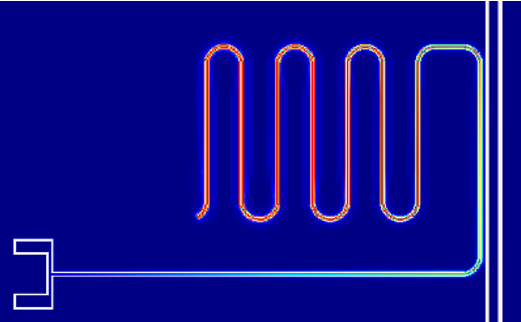
\includegraphics[height=0.3\textheight]{xmonres_sim_claw_h}
		
		\hspace{-2cm}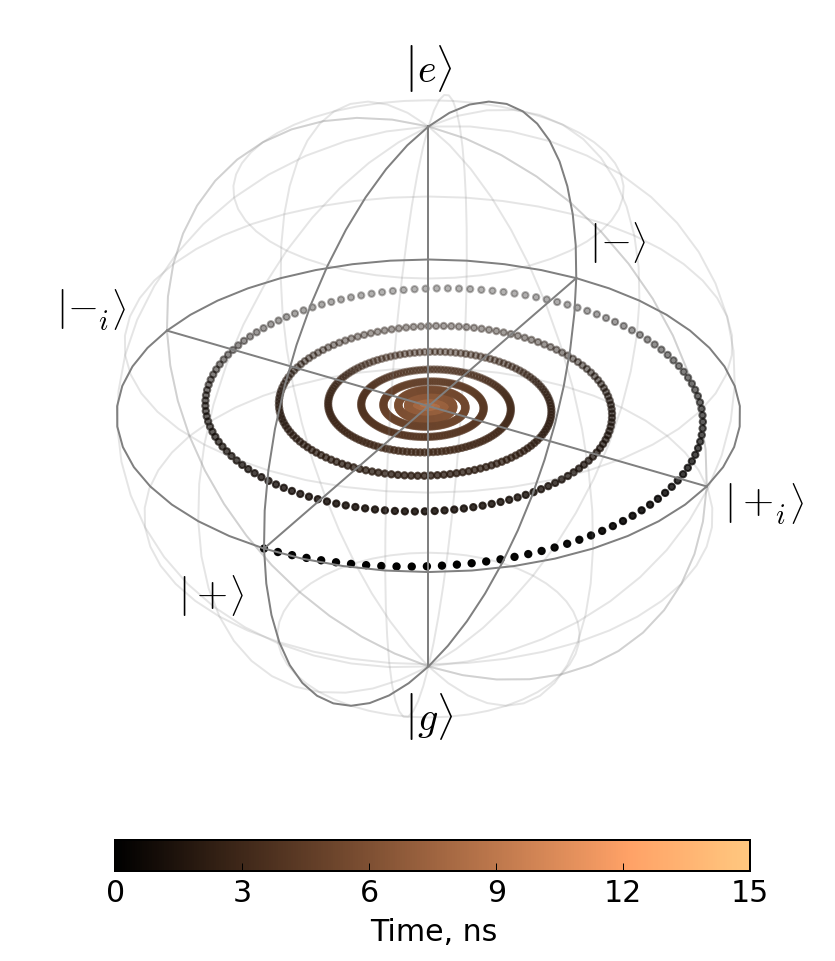
\includegraphics[height=0.3\textheight]{qdeph_bloch}
    
    	\hspace{-2cm}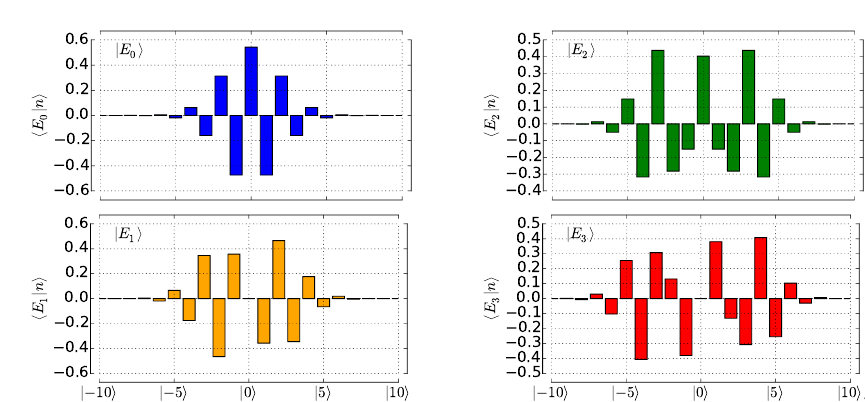
\includegraphics[height=0.3\textheight]{tr_CPD}

  \end{columns}
}
\addtocounter{page}{-1}

\AtBeginSection[]
{
  \begin{frame}[plain]
    \tableofcontents[currentsection]
    \addtocounter{page}{-1}
  \end{frame}
}
\subsection{Quality factors and effective parameters}
\begin{frame}[t]\frametitle{\secname}\framesubtitle{\subsecname}

Capacitively coupled CPW resonator as a lumped-element model: 

\vspace{0.5cm}
\begin{columns}[c]
\onslide<1,2,3>{
	\column{0.45\textwidth}
	\centering
	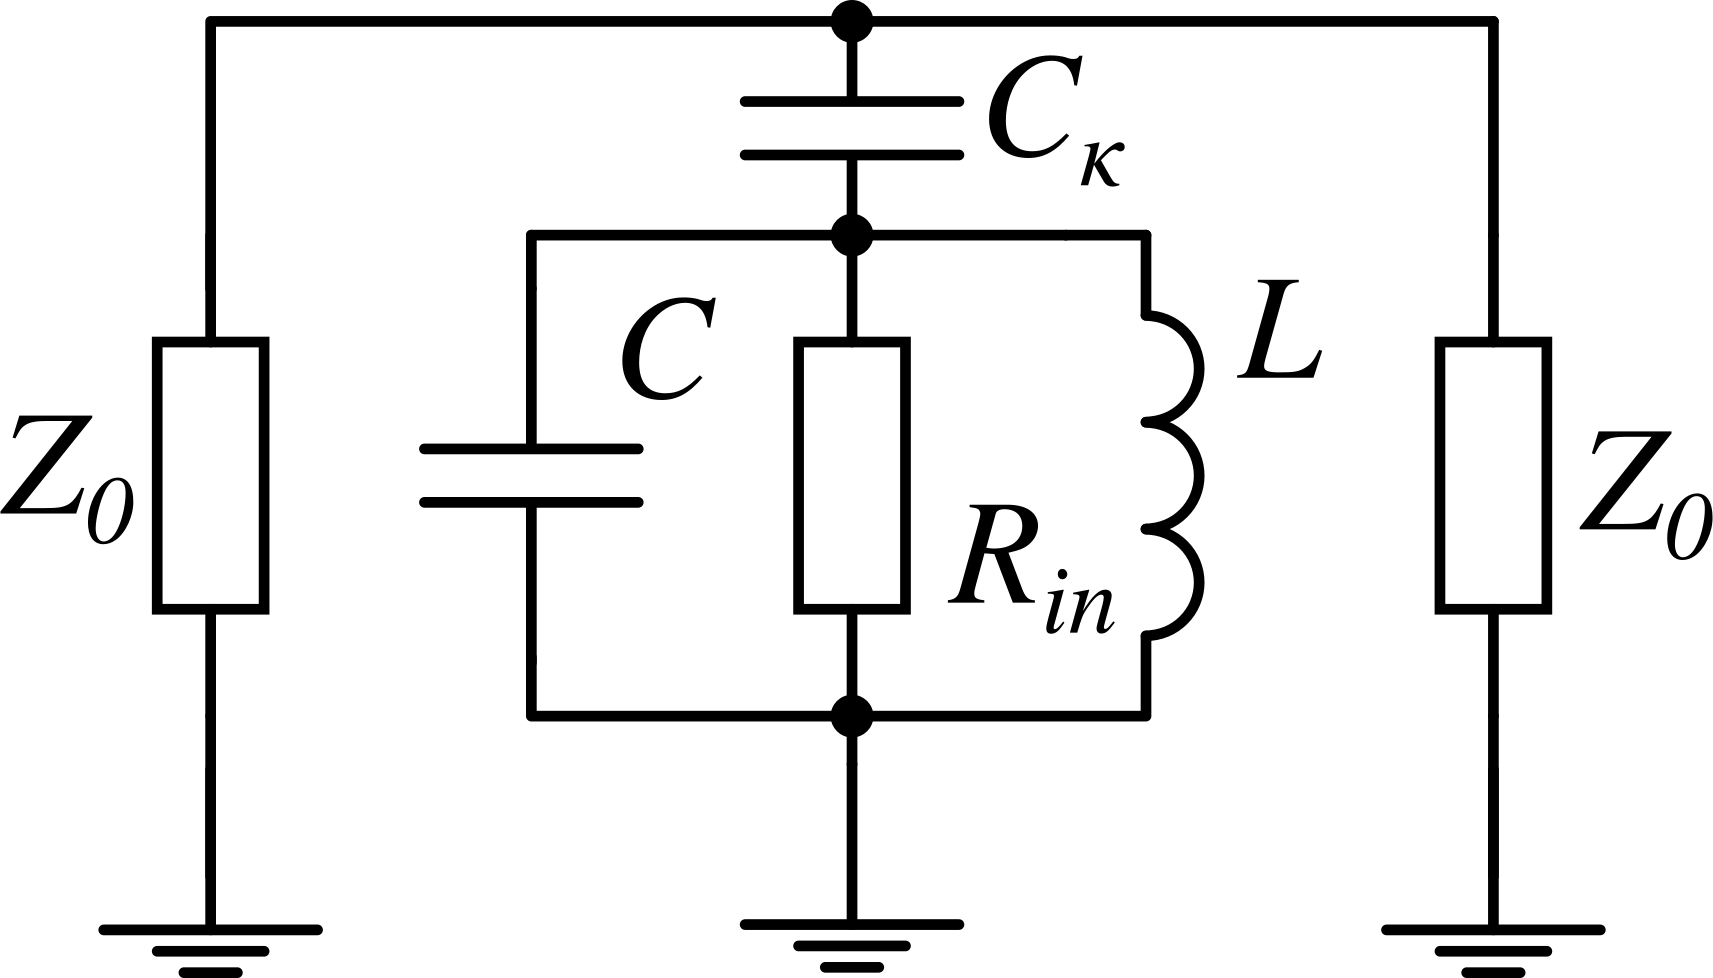
\includegraphics[width=0.9\textwidth]{resonator}

}
\onslide<2,3>{
	\column{0.1\textwidth}
	\centering
	{ \Huge $\Leftrightarrow$ }
\column{0.45\textwidth}

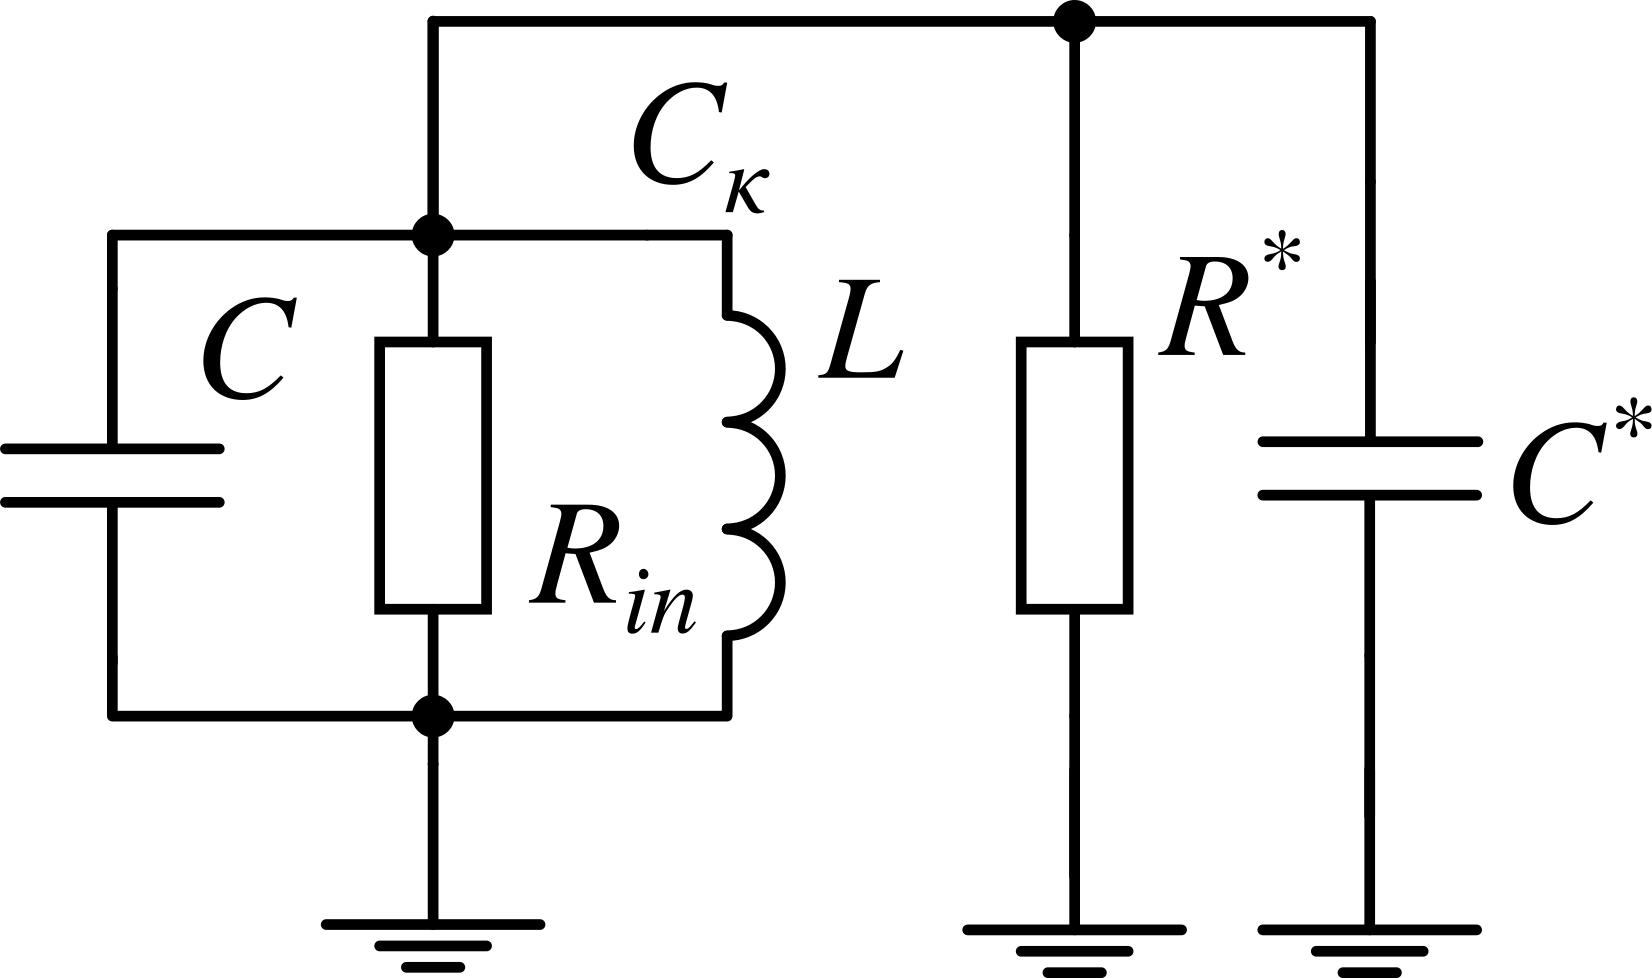
\includegraphics[width=0.9\textwidth]{resonator_equiv}
}
\end{columns}
\only<1>{
	
	\vspace{2cm}
}
\only<2>{
\vspace{0.5cm}
	\[
	R^{*} = \frac{1+\omega^2 C_\kappa^2 (Z_0/2)^2}{\omega^2 C_\kappa^2 (Z_0/2)	}, \quad
	C^{*} = \frac{C_\kappa}{1+\omega^2 C_\kappa^2 (Z_0/2)^2} \approx C_\kappa\ (\text{for our case}). 
	\]
}
\only<3>{
\vspace{0.5cm}
	\[
	Q_i =  \omega (C+C^{*}) R_{in}, \quad
	Q_e = \omega (C+C^{*}) R^{*}, \quad
	Q_l = \omega (C+C^{*})  \frac{1}{1/R^{*}+1/R_{in}}. 
\]
}
\end{frame}

\frame{\frametitle{\secname}\framesubtitle{\subsecname}
Q-factors depending on $C_\kappa$:

\centering

\vspace{0.5cm}
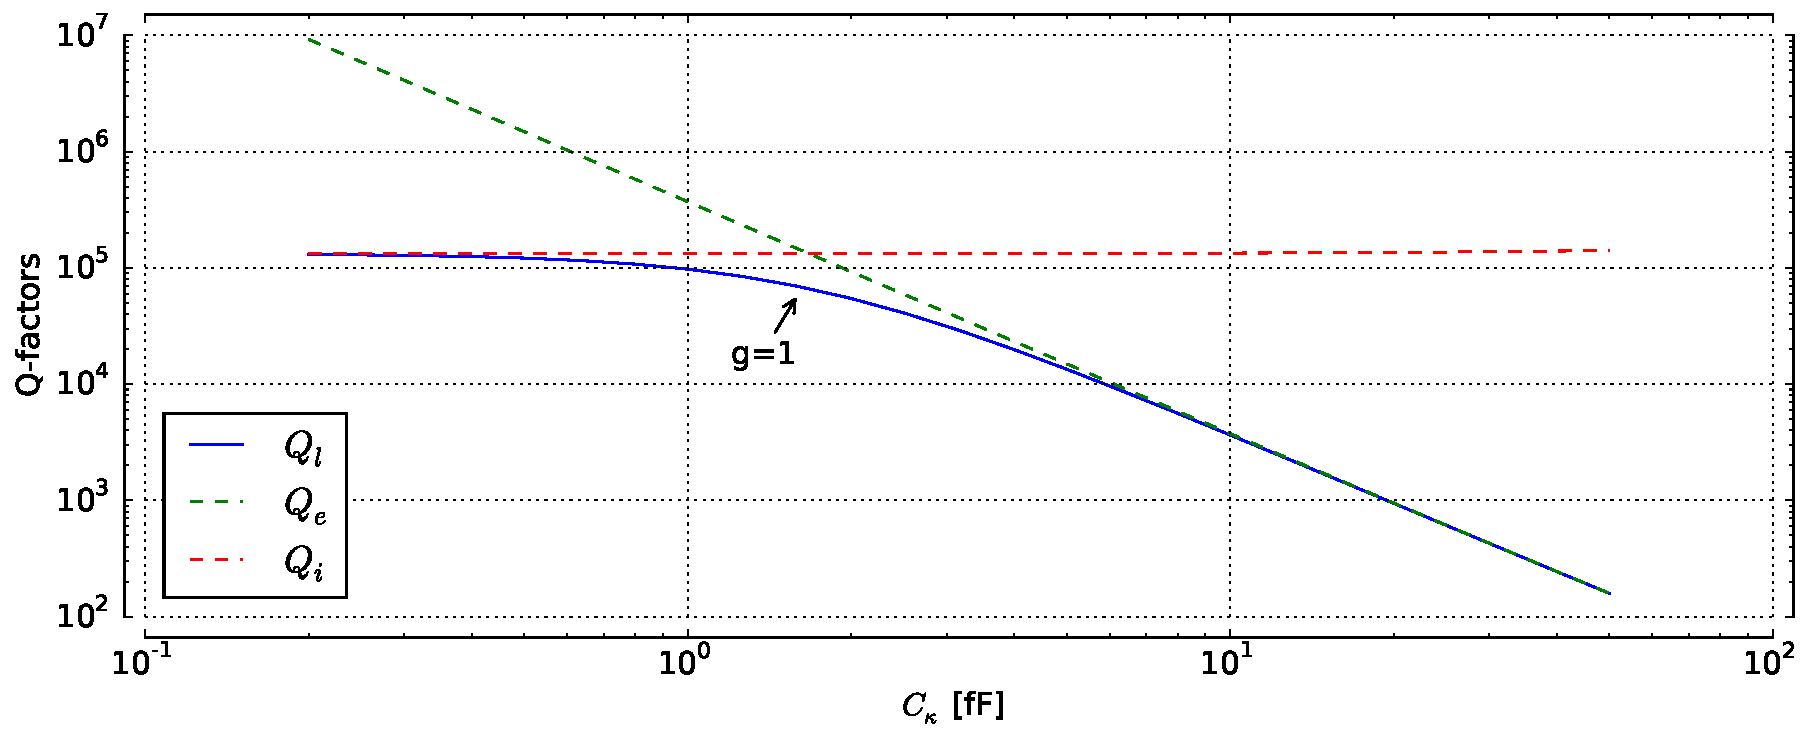
\includegraphics[width=\textwidth]{q-factors}
}

\subsection{S-parameters}
\begin{frame}[t]\frametitle{\secname}\framesubtitle{\subsecname}

General algorithm for calculating S-parameters of a given device:

\vspace{0.5cm}
\begin{columns}[c]
\column{0.5\textwidth}
\centering

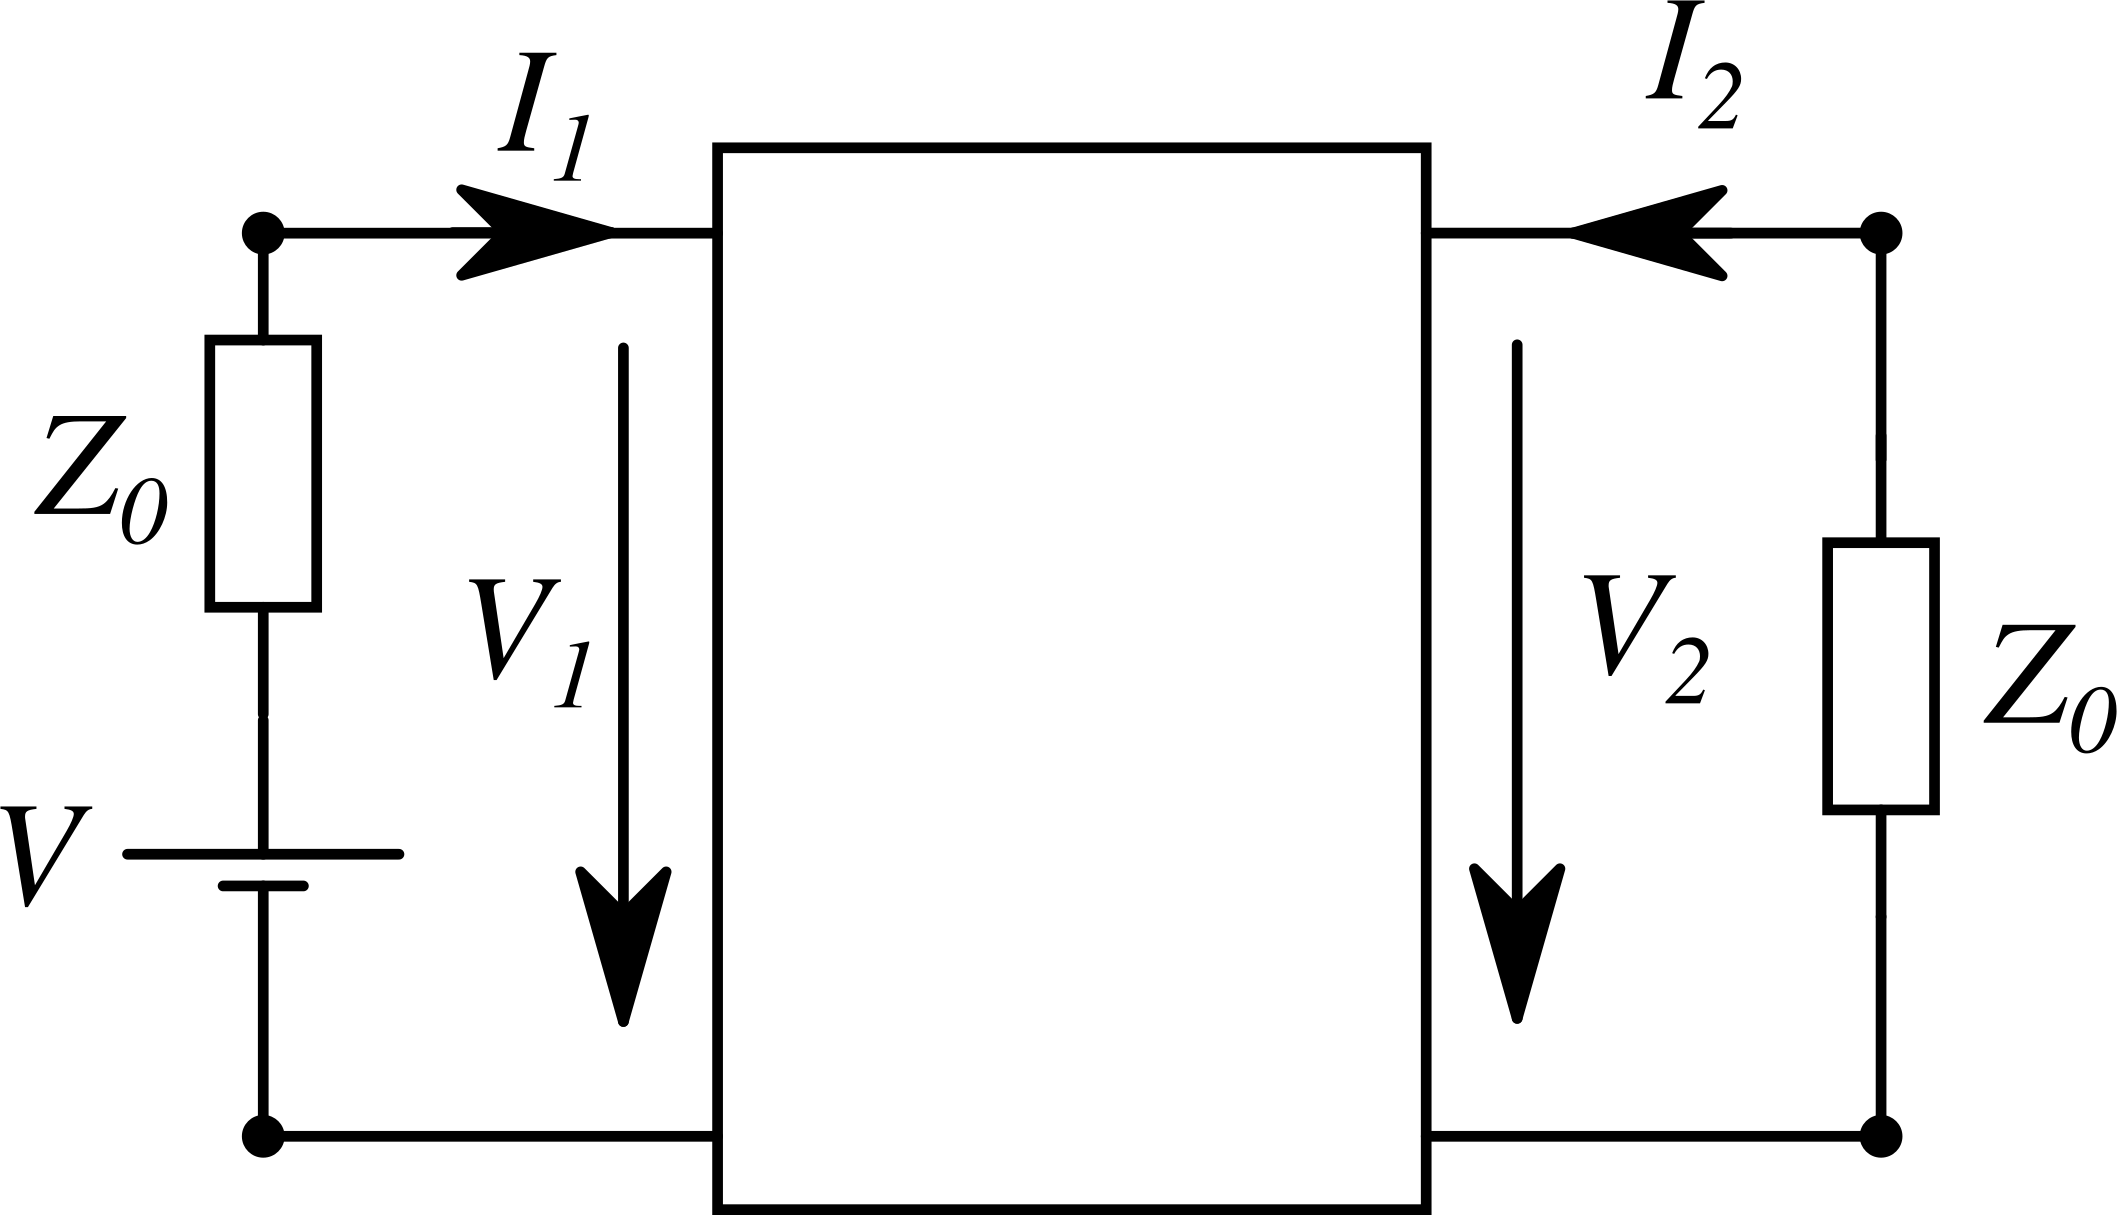
\includegraphics[width=0.95\textwidth]{tl_scheme_general}
\column{0.5\textwidth}
\centering

\vspace{0.35cm}
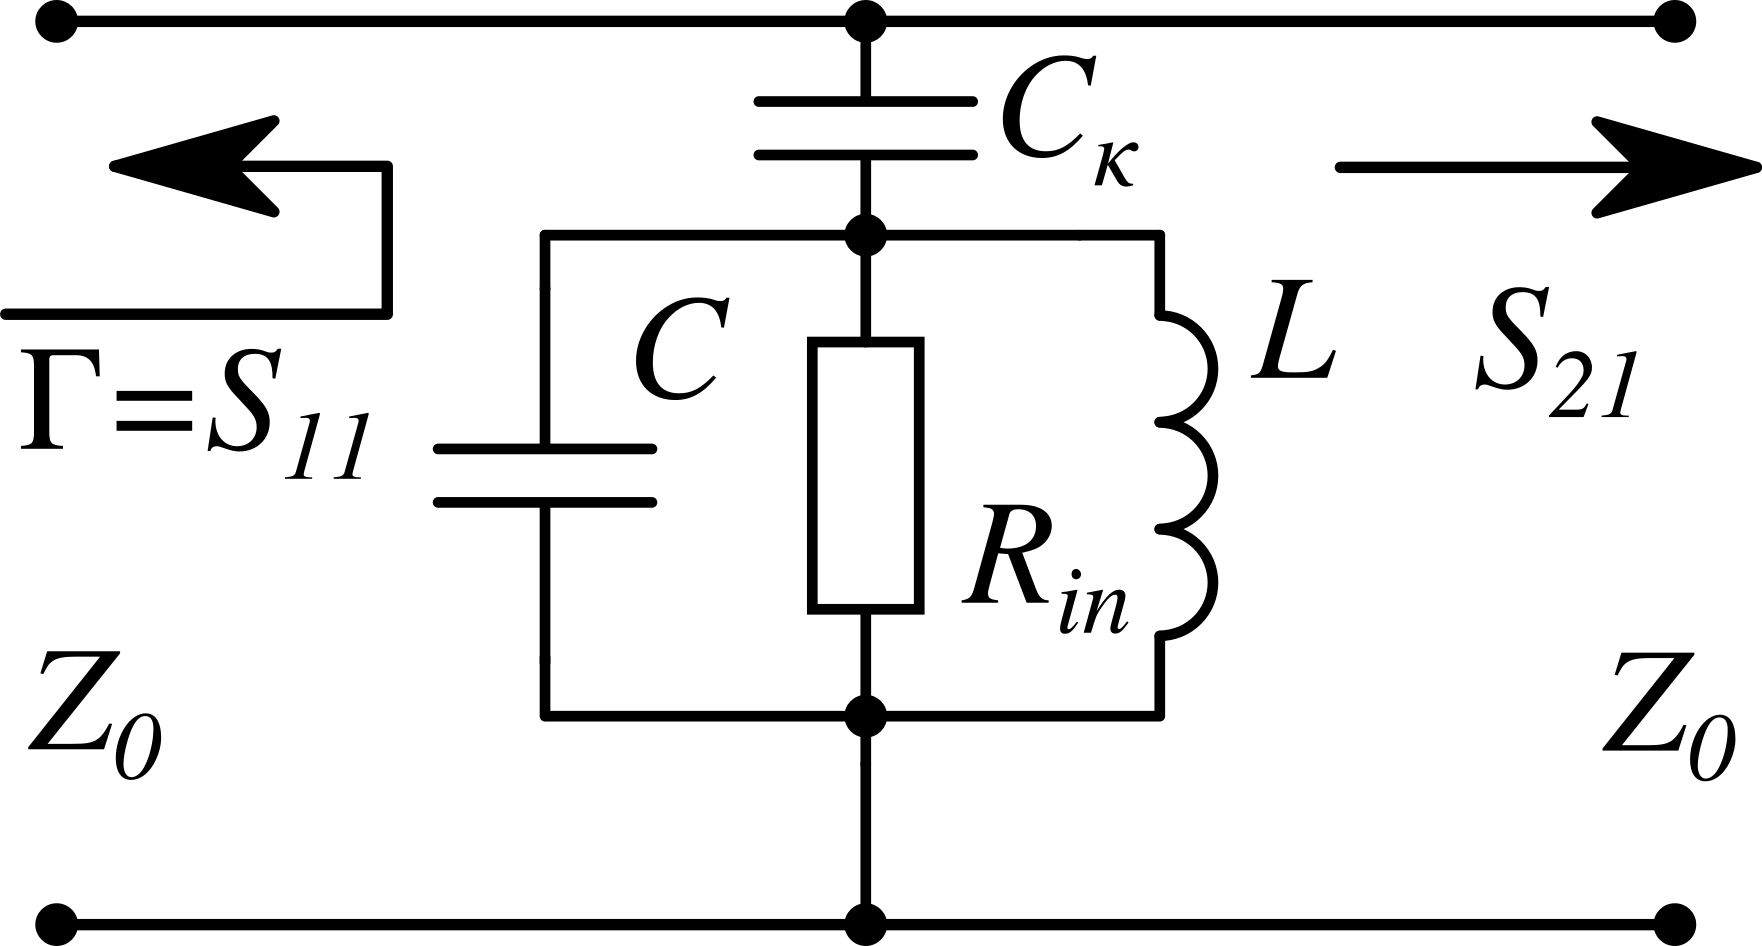
\includegraphics[width=0.8\textwidth]{tl_scheme}
\end{columns}

\begin{equation*}
\text{Kirchgoff's laws}\quad \Rightarrow \quad
\begin{gathered}
V_{1,2} = V_{1,2}^+ + V_{1,2}^- ,\\
I_{1,2} = \frac{ V_{1,2}^+ - V_{1,2}^- }{Z_0}
\end{gathered} \quad \Rightarrow \quad
\rbrkt{\begin{matrix}
V_1^- \\
V_2^-
\end{matrix}} = 
\rbrkt{\begin{matrix}
S_{11} & S_{12} \\
S_{21} & S_{22}
\end{matrix}}
\rbrkt{\begin{matrix}
V_1^+ \\
V_2^+
\end{matrix}}.
\end{equation*}

\end{frame}

\frame{\frametitle{\secname}\framesubtitle{\subsecname}
Analytical $S_{21}(C_\kappa, \omega) = (1+Z_0/2Z_{sh})^{-1},\ Z_{sh} = 1/i\omega C_\kappa + Z_{res}$:

\centering
\vspace{0.5cm}
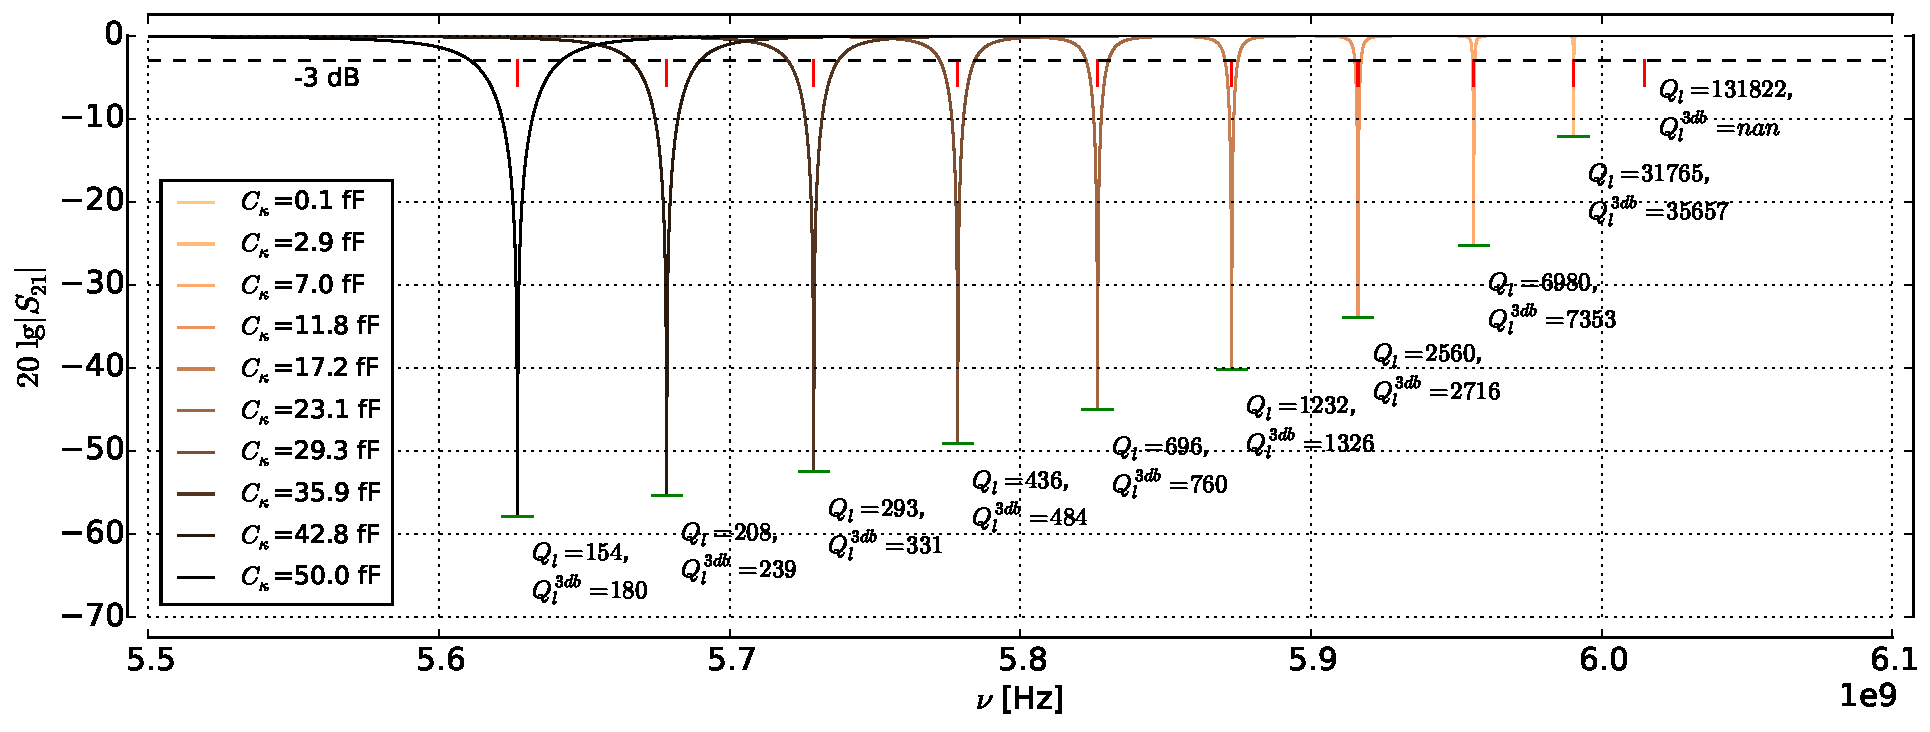
\includegraphics[width=\textwidth]{S21s}
}

\subsection{Xmon design features}
\begin{frame}[c]\frametitle{\secname}\framesubtitle{\subsecname}
\begin{columns}[c]
\column{0.3\textwidth}
{\footnotesize Designed in LayoutEditor}

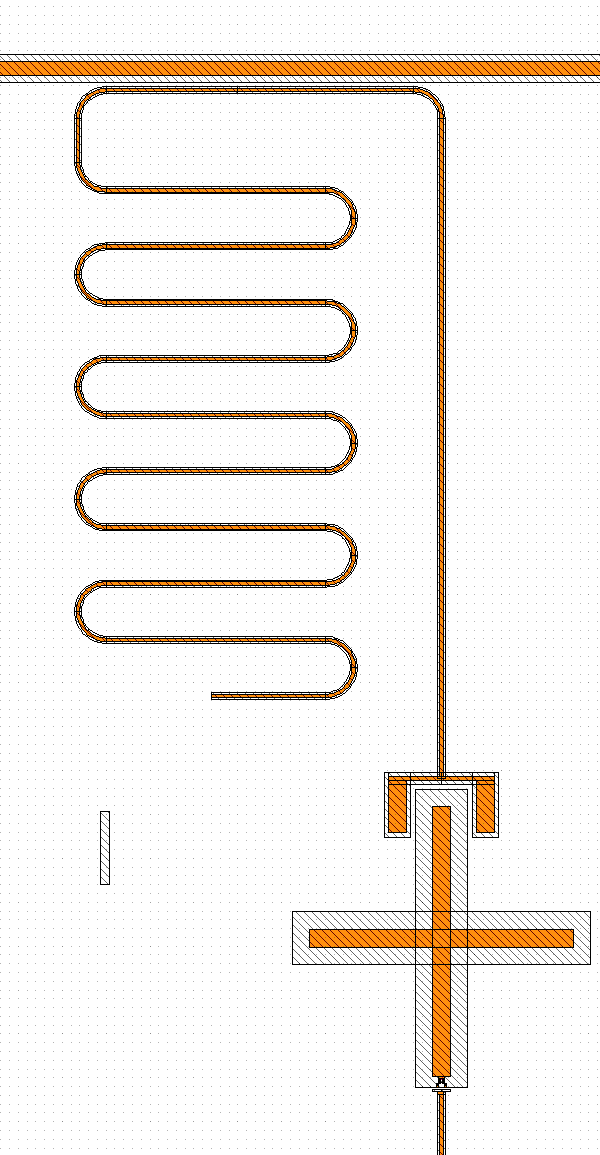
\includegraphics[height=0.85\textheight]{xmonres}
\column{0.7\textwidth}
$l = \lambda/4$ coplanar resonators, $W=4\,\mu m,\ G=2\,\mu m$.

\vspace{0.5cm}
Unconventional coupling to the feedline:
 $$C_\kappa^{eff} = C_\kappa \cos \frac{\pi x_\kappa}{2 l}\ ? \text{ [1]}$$
 $$M_\kappa =\ ?$$
``Claw'' coupler at the open end. Adds up some phase $\phi(\omega)$ and can be replaced [1] with high accuracy by
$$\Delta l = \frac{\phi(\omega_r) c}{2 \omega_r \sqrt{\varepsilon_{eff}}}$$


{\footnotesize[1] D. Sank, PhD Thesis, 2014}
\end{columns}
\end{frame}


\subsection{Sonnet simulations}
\begin{frame}[t]\frametitle{\secname}\framesubtitle{\subsecname}
\only<1>{
	Resonator without a claw. Frequency expected from the length and $C_\kappa\approx 6$ fF (extracted from $Q_l \approx 10^4$) is 7.925 GHz.

	\vspace{0.2cm}
	\begin{columns}[c]
	\column{0.4\textwidth}
	\centering
	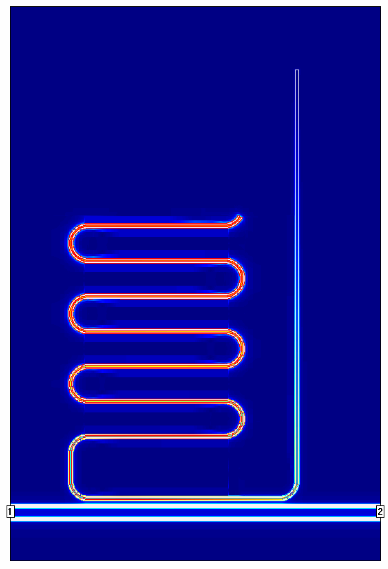
\includegraphics[height=0.7\textheight]{xmonres_sim_noclaw}
	\column{0.6\textwidth}
	\centering
	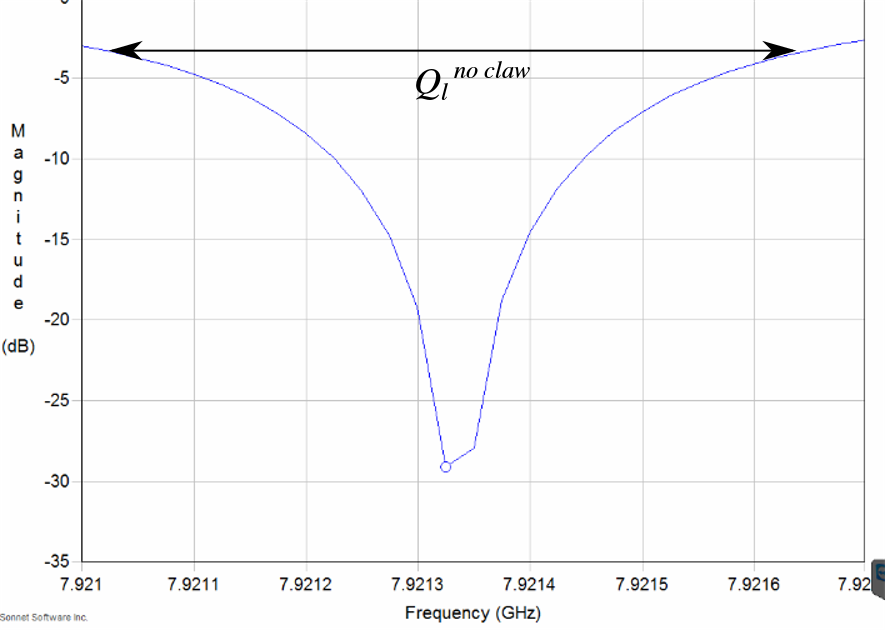
\includegraphics[width=\textwidth]{xmonres_sim_noclaw_res}
	\end{columns}
}
\only<2>{
	Resonator with a claw. Frequency expected from the previous simulation and $\phi$ (also simulated separately for the given claw) is 7.4255 GHz.
	
	\vspace{0.2cm}
	\begin{columns}[c]
	\column{0.4\textwidth}
	\centering
	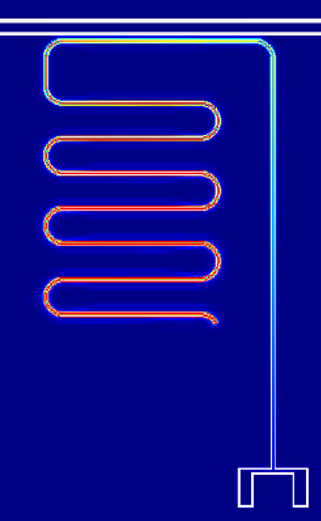
\includegraphics[height=0.7\textheight]{xmonres_sim_claw}
	\column{0.6\textwidth}
	\centering
	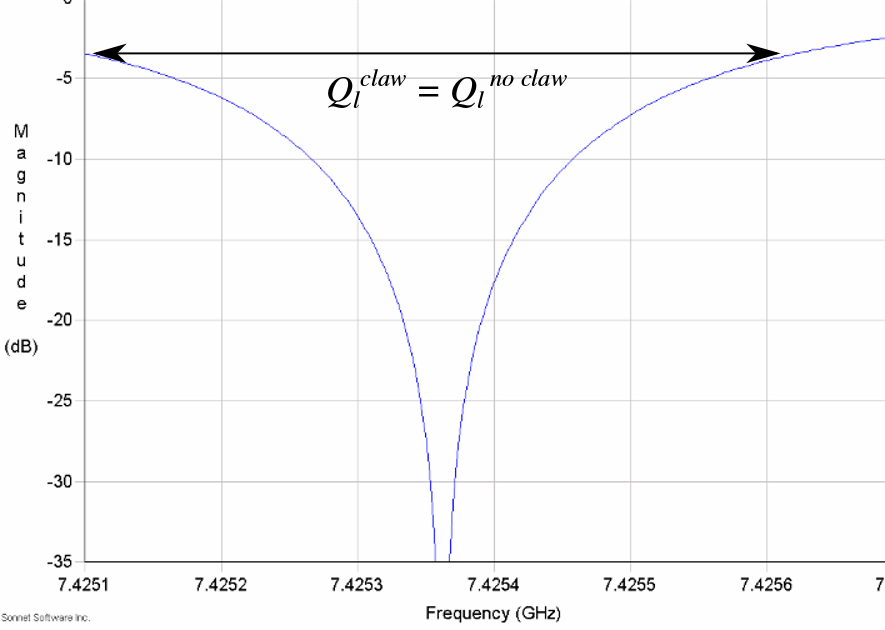
\includegraphics[width=\textwidth]{xmonres_sim_claw_res}
	\end{columns}
}

\end{frame}

\section{Noise and decoherence versus Hahn echo technique}
\subsection{Quantum-mechanically treated pure dephasing (Ramsey)}
\frame{\frametitle{\secname}\framesubtitle{\subsecname}
\only<1> {
	Qubit-environment interaction Hamiltonian:
	\[
	\mathcal{\hat H}_{qe} = \hat O_e \otimes  \hat \sigma_z.
	\]
	$\hat O_e$ is an arbitrary environment operator, $\hat \sigma_z$ -- qubit observable.
	
	~
	
	 Master equation:
	\[
	\partial_t \hat \rho_q = \frac{i}{\hbar}[\hat \rho_s, \mathcal{\hat H}_s] + \gamma_\phi (\hat \sigma_z \hat \rho_s \hat \sigma_z - \hat \rho_s).
	\]
	Steady state:
	\[
	\hat \rho_q (\infty) = \rbrkt{\begin{matrix}
	\rho_{11}(0) & 0 \\
	0 & \rho_{22}(0) 
	\end{matrix}}.
	\]
}
\only<2>{
	Example: pure dephasing of the $\ket{+}$  state, \bf lab frame.
	\begin{columns}[c]
	\column{0.4\textwidth}
	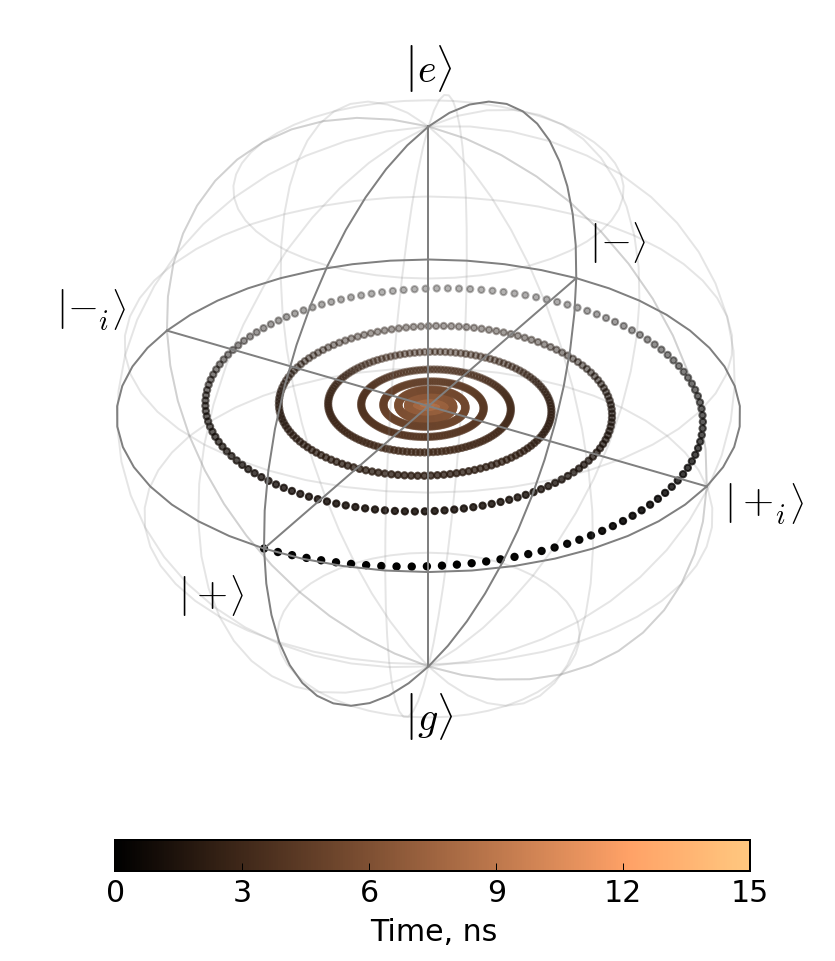
\includegraphics[width=\textwidth]{qdeph_bloch}
	\column{0.6\textwidth}
	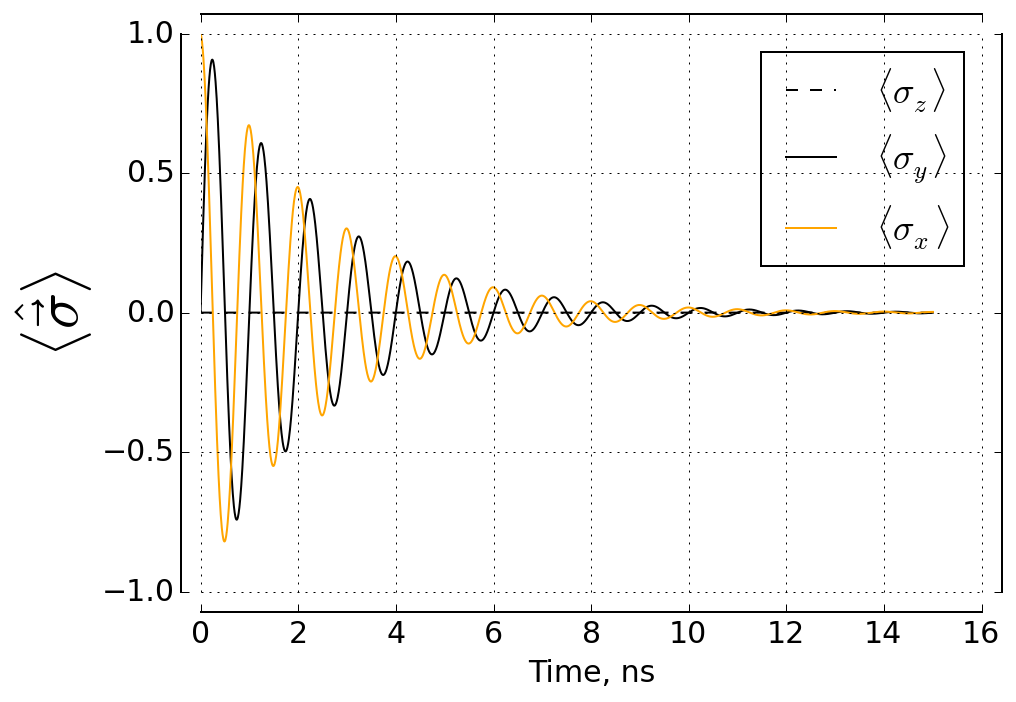
\includegraphics[width=\textwidth]{qdeph_xyz}
	\end{columns}
}
\only<3>{
	Example: pure dephasing of the $\ket{+}$  state, \bf rotating frame.

	\begin{columns}[c]
	\column{0.4\textwidth}
	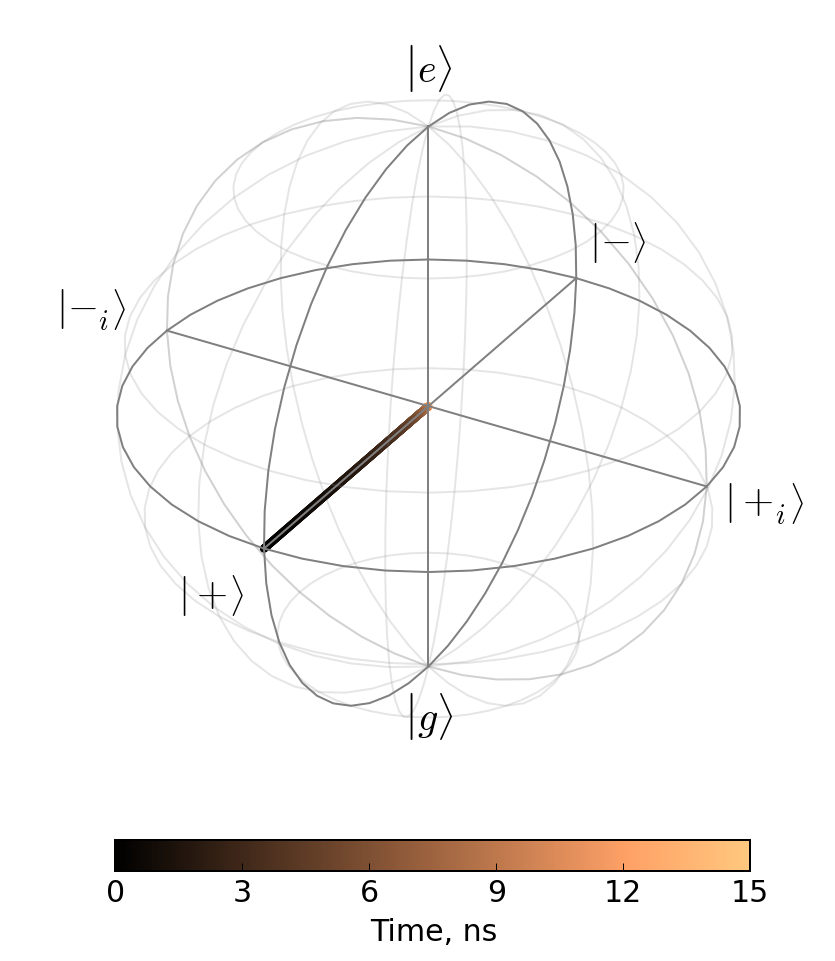
\includegraphics[width=\textwidth]{qdeph_bloch_rf}
	\column{0.6\textwidth}
	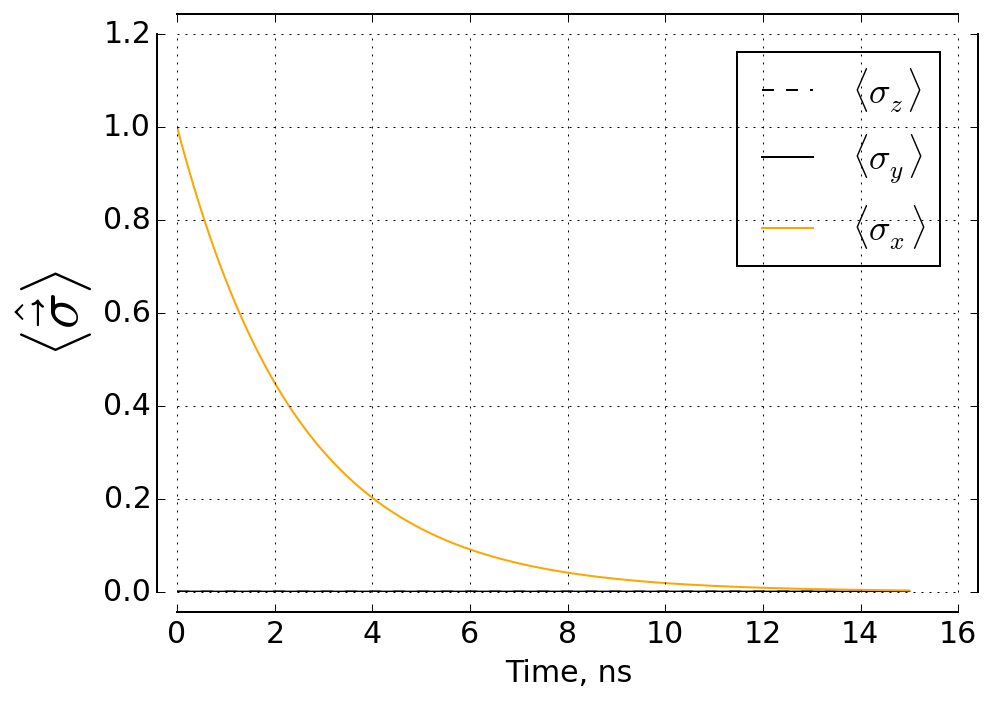
\includegraphics[width=\textwidth]{qdeph_xyz_rf}
	\end{columns}
}
}
\subsection{Classically treated pure dephasing (Ramsey)}
\frame{\frametitle{\secname}\framesubtitle{\subsecname}
\only<1>{
	$$\hat O_e \otimes \hat  \sigma_z \rightarrow f(t) \cdot \hat \sigma_z,\ f(t)\ \text{is random}$$ 
	
	Rotating frame evolution:
	\[
	\hat \rho_q (t) = \hat U^\dag(t, 0)\ \hat\rho_q(0)\ \hat U(t, 0), \quad \hat U(t, 0) = \hat T \exp \left\{-\frac{i}{\hbar} \int_0^t f(\tau)\hat \sigma_z \diff\tau\right\}.
	\]
	\[
	\hat \rho_q (t) = \rbrkt{\begin{matrix}
	1/2 - N(t)/2 & \rho(t) \\
	\rho^*(t) & 1/2 + N(t)/2 
	\end{matrix}},
	\]
	\begin{mybox}
	\[
	\left. \begin{gathered}
	N(t) = N(0),\\
	\rho(t) = \rho(0)\exp \left\{ \frac{2i}{\hbar}\int_0^t f(\tau)  \diff \tau \right\} 
	\end{gathered}\right\}
	 \Rightarrow \begin{matrix} \text{\bf unitary random walk,}\\ \text{\bf no dephasing!}\end{matrix}
	\]
	\end{mybox}
}
\only<2>{
	\textbf{Averaging.} For Gaussian instantaneous distribution of $f(t),\ \frac{2}{\hbar}\int_0^t f(\tau) \diff \tau$:
	\begin{gather*}
	\langle \rho(t) \rangle = \rho(0)\exp \left\{ -\frac{2}{\hbar^2}\int_0^t\int_0^t \langle f(\tau_1) f(\tau_2) \rangle \diff\tau_1 \diff \tau_2 \right\}.
	\end{gather*}
	Presuming also that $f(t)$ is a wide-sense stationary process: $$\langle f(\tau_1) f(\tau_2) 				\rangle = K_f(\tau_2 - \tau_1) = \frac{1}{\sqrt{2\pi}}\int\limits_{-\infty}^{\infty} S_f(\omega) e^{i\omega(\tau_2-\tau_1)}\diff\omega.$$ 
	\begin{mybox}
	\[
	\langle \rho(t) \rangle = \rho(0) \exp  \left\{-\frac{2}{\sqrt{2\pi}\hbar^2} \int\limits_{-\infty}^{\infty}  \frac{4 \sin^2(\frac{\omega t}{2})}{\omega^2} S_f(\omega)\diff \omega \right\} \equiv \rho(0)e^{-\alpha (t)}
	\]
	\centering
	$\Rightarrow$ \bf  ensemble averaged behaviour is non-unitary!
	\end{mybox}
}
}

\subsection{Hahn echo}
\begin{frame}[t]\frametitle{\secname}\framesubtitle{\subsecname}
\textbf{Add one instant $\pi$-pulse}. Accumulated phase:
\begin{equation*}
\rho(t) = \rho(0)\exp \Big\{ \underbrace{- \frac{2i}{\hbar}\int_0^{t/2} f(\tau)  \diff \tau}_{\text{before }\pi\text{-pulse}} + \underbrace{\frac{2i}{\hbar}\int_{t/2}^{t} f(\tau)  \diff \tau}_{\text{after }\pi\text{-pulse}} \Big	\}.
\end{equation*}
After averaging:
\begin{mybox}
\[
\begin{gathered}
\left<\rho(t)\right> = \rho(0)\exp \Big\{ - \frac{2}{\sqrt{2\pi} \hbar^2} \int\limits_{-\infty}^{\infty}  S_f(\omega) W_t (\omega)\diff \omega \Big\},\\
W_t (\omega) = \tan^2(\omega t/4)\frac{4 \sin^2(\omega t/2)}{\omega^2}.
\end{gathered}
\]
\end{mybox}
\end{frame}

\subsection{Noise PSD filtration}
\begin{frame}[t]\frametitle{\secname}\framesubtitle{\subsecname}
\begin{columns}[c]
\column{0.5\textwidth}
\centering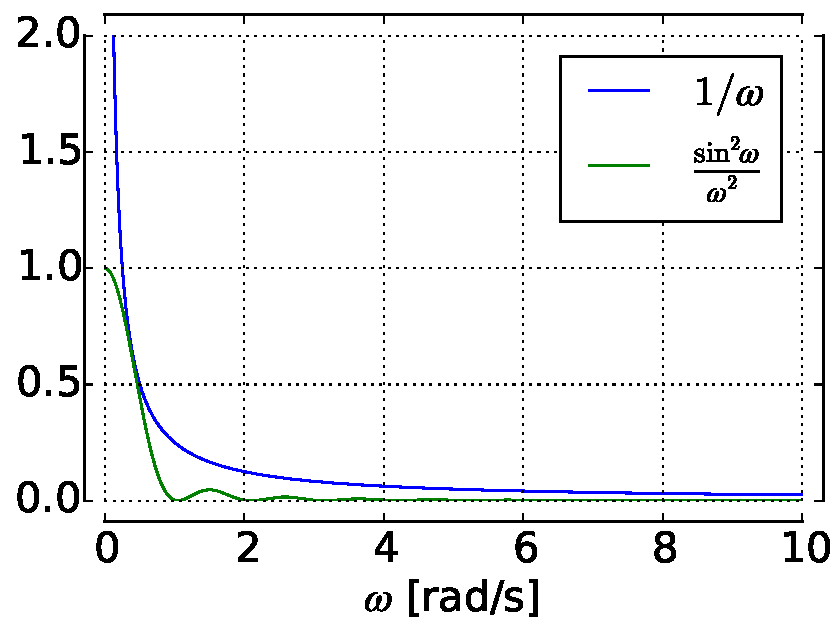
\includegraphics[width=\textwidth]{ramsey_filter}

\vspace{0.1cm}
\begin{itemize}
\item Ramsey: $\int  \frac{4 \sin^2(\frac{\omega t}{2})}{\omega^2} S_f(\omega)\diff \omega $ 
\end{itemize}
\column{0.5\textwidth}
\centering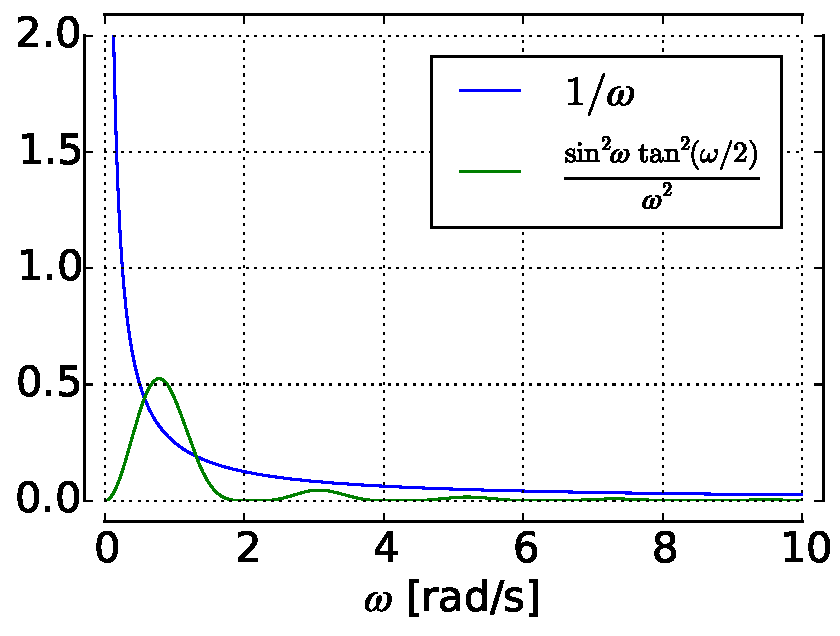
\includegraphics[width=\textwidth]{hahn_filter}

\vspace{0.1cm}
\begin{itemize}

\item Hahn: $\int \tan^2(\omega t/4) \frac{4 \sin^2(\frac{\omega t}{2})}{\omega^2} S_f(\omega)\diff \omega  $ 

\end{itemize}
\end{columns}

\end{frame}

\subsection{Who wins?}
\begin{frame}[t]\frametitle{\secname}\framesubtitle{\subsecname}
$S_f(\omega) = \delta(\omega)$ ($f(t) = const$ in each single run):
\only<1>{

	\vspace{10cm}
	\vfill
}
\only<2>{

	\vspace{0.2cm}
	\begin{columns}[c]
	\column{0.4\textwidth}
	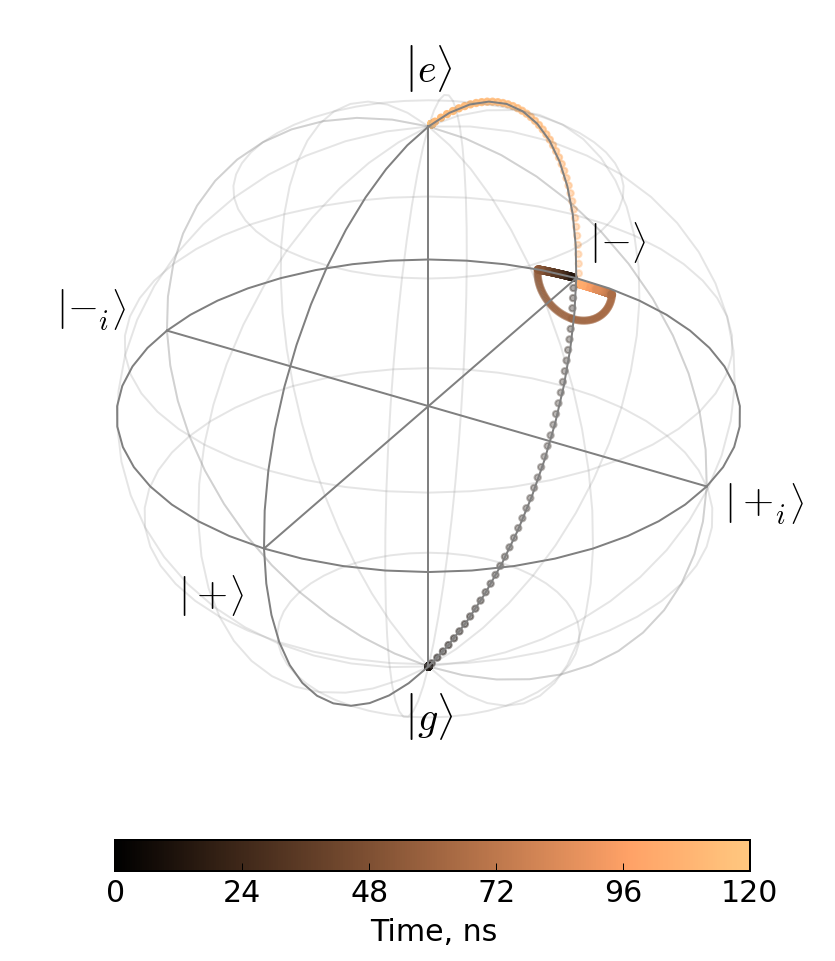
\includegraphics[width=\textwidth]{cse_bloch_rf}
	\column{0.6\textwidth}
	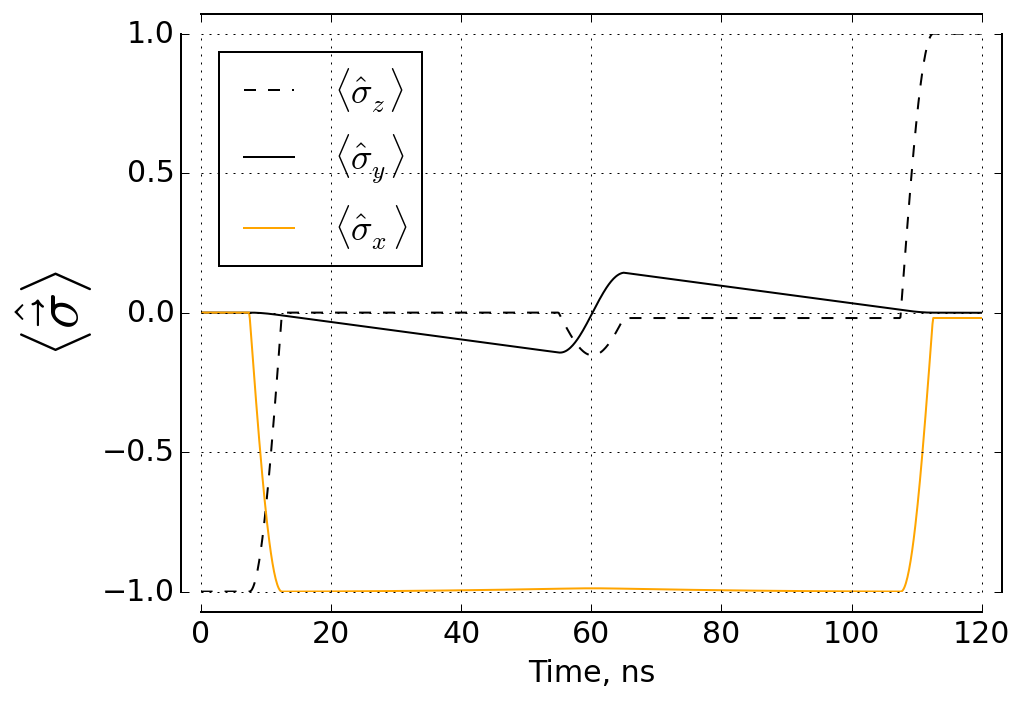
\includegraphics[width=\textwidth]{cse_xyz_rf}
	
	
	\vspace{-0.3cm}
	\begin{itemize}
	\centering	
	\item \bf full efficiency for instant pulses
	\end{itemize}
	\end{columns}
}
\end{frame}


\begin{frame}[t]\frametitle{\secname}\framesubtitle{\subsecname}
$S_f(\omega) =1/\omega$ (pink noise):
\only<1>{

	\vspace{0.2cm}
	\begin{columns}[c]
	\column{0.5\textwidth}
	\centering
	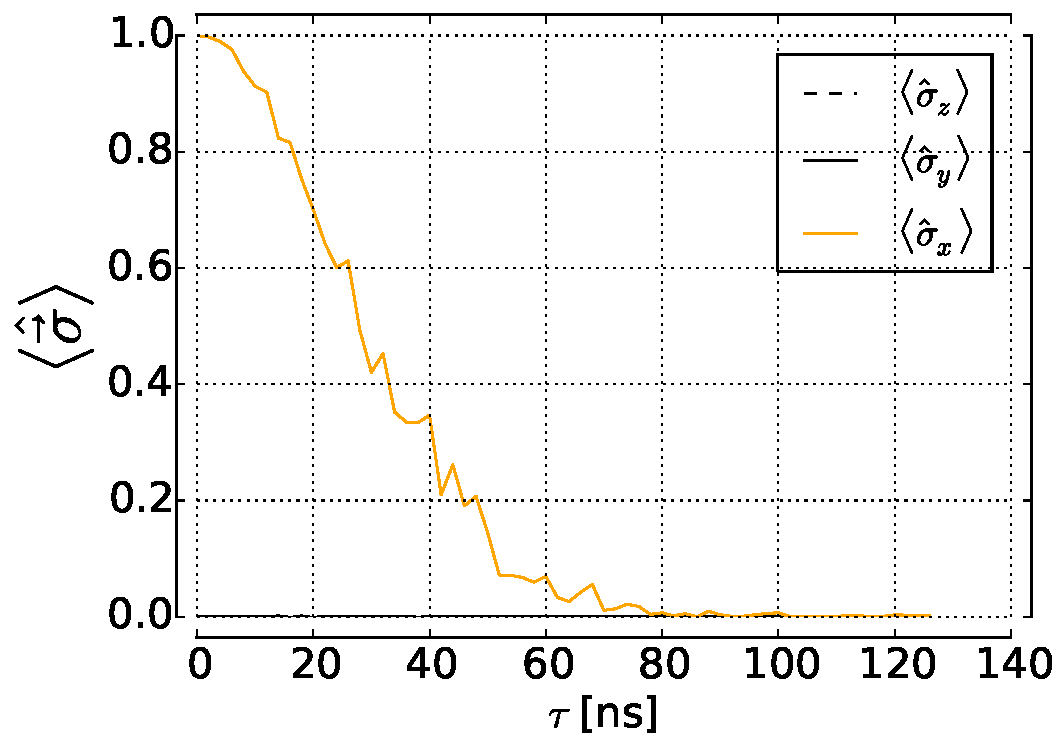
\includegraphics[width=\textwidth]{deph_pink}
	
	No echo
	\column{0.5\textwidth}
	\vfill
	\end{columns}
}
\only<2>{

	\vspace{0.2cm}
	\begin{columns}[c]
	\column{0.5\textwidth}
	\centering
	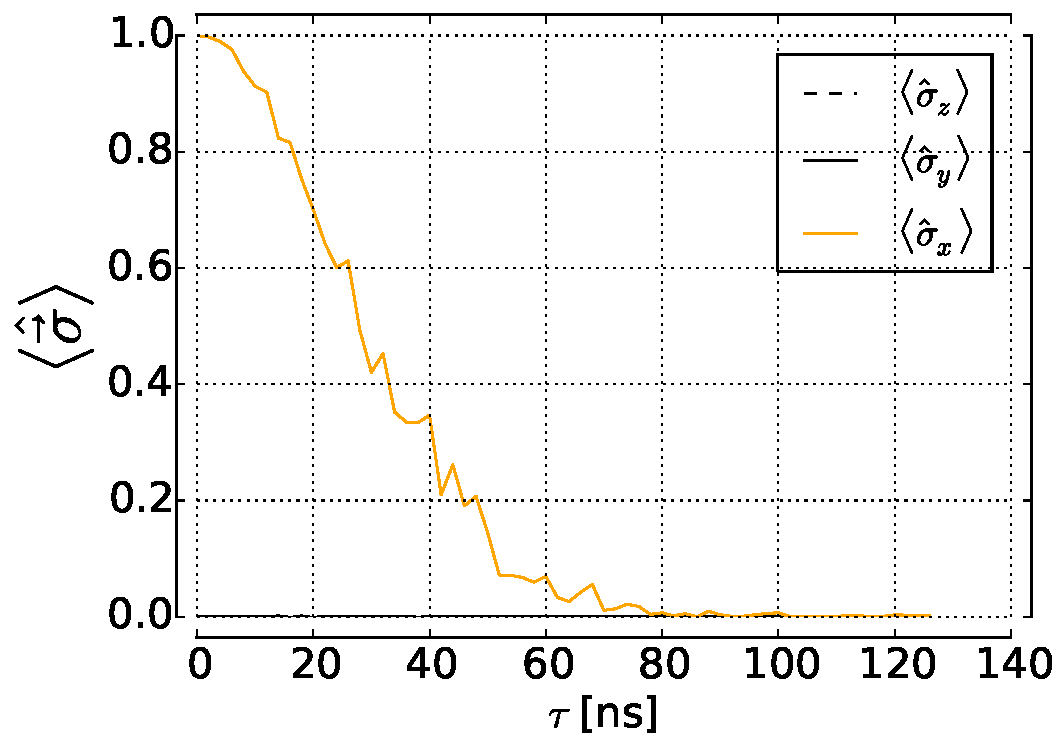
\includegraphics[width=\textwidth]{deph_pink}
	
	No echo
	\column{0.5\textwidth}
	\centering
	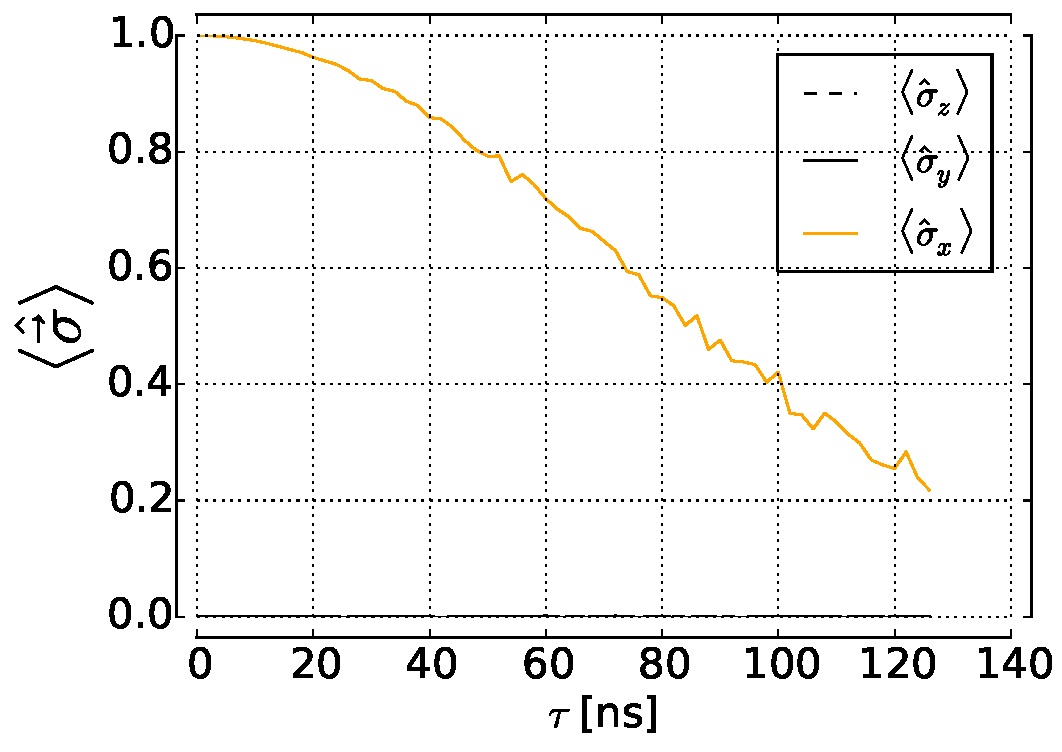
\includegraphics[width=\textwidth]{deph_pink_se}
	
	Echo
	\end{columns}
	
	
	\vspace{0.2cm}
	\begin{itemize}
	\centering	
	\item \bf efficient!
	\end{itemize}
}
\end{frame}

\begin{frame}[t]\frametitle{\secname}\framesubtitle{\subsecname}
$S_f(\omega) =S_f(0) = const$ (white noise):
\only<1>{

	\vspace{0.2cm}
	\begin{columns}[c]
	\column{0.5\textwidth}
	\centering
	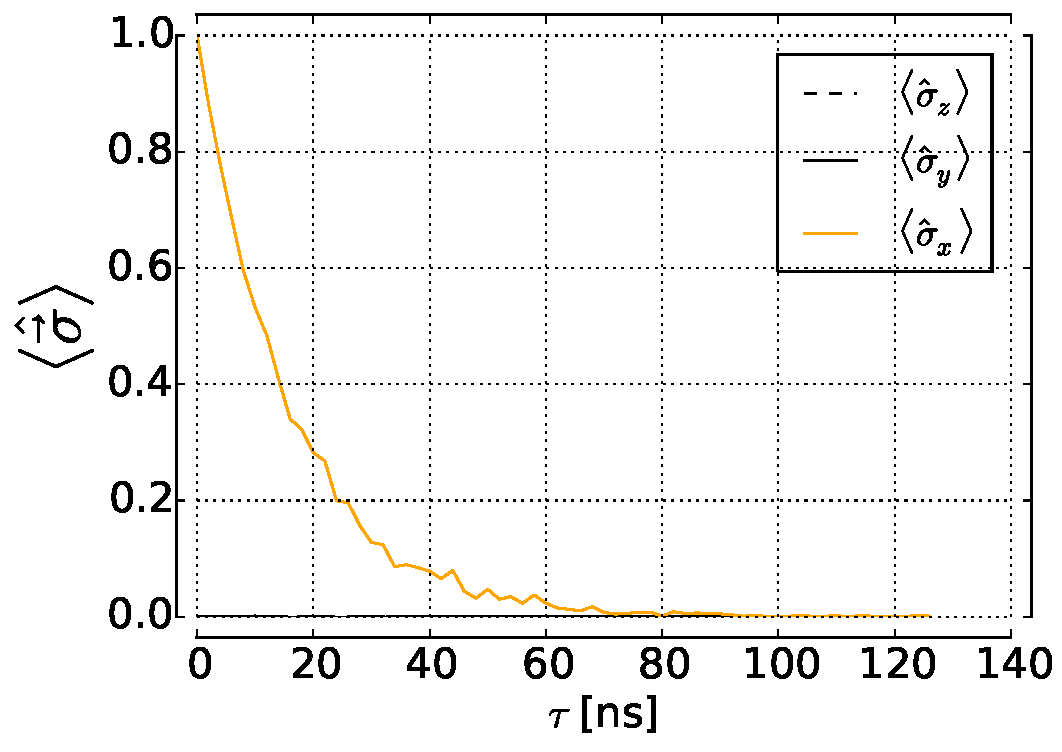
\includegraphics[width=\textwidth]{deph_white}
	
	No echo
	\column{0.5\textwidth}
	\vfill
	\end{columns}
}
\only<2>{

	\vspace{0.2cm}
	\begin{columns}[c]
	\column{0.5\textwidth}
	\centering
	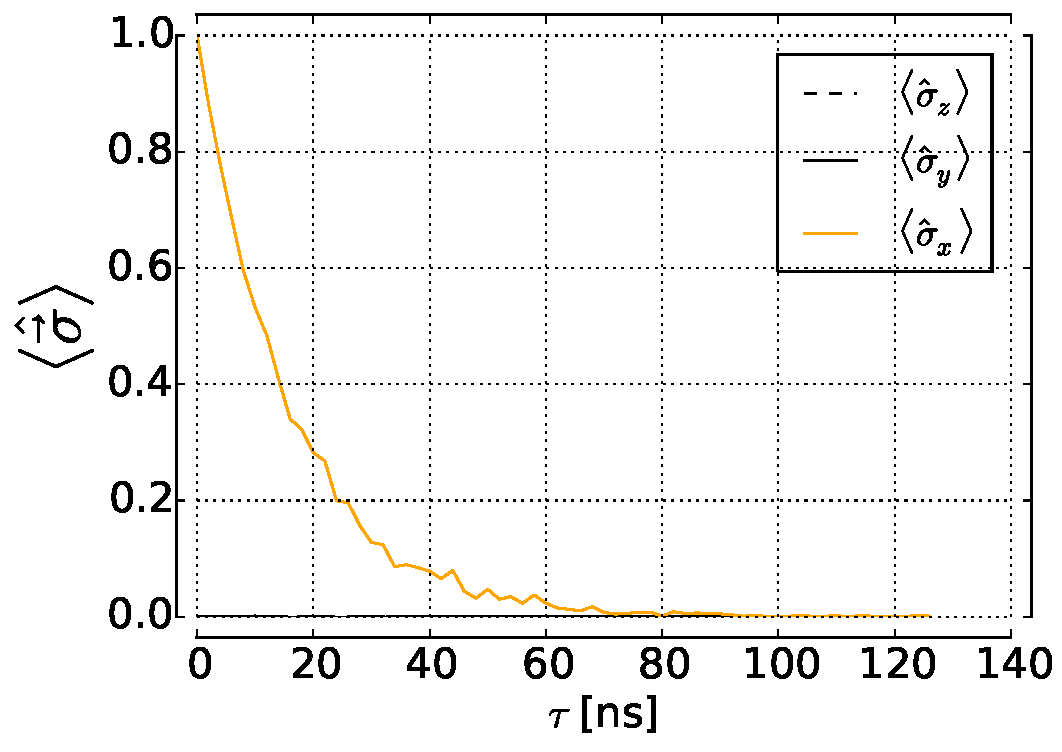
\includegraphics[width=\textwidth]{deph_white}
	
	No echo
	\column{0.5\textwidth}
	\centering
	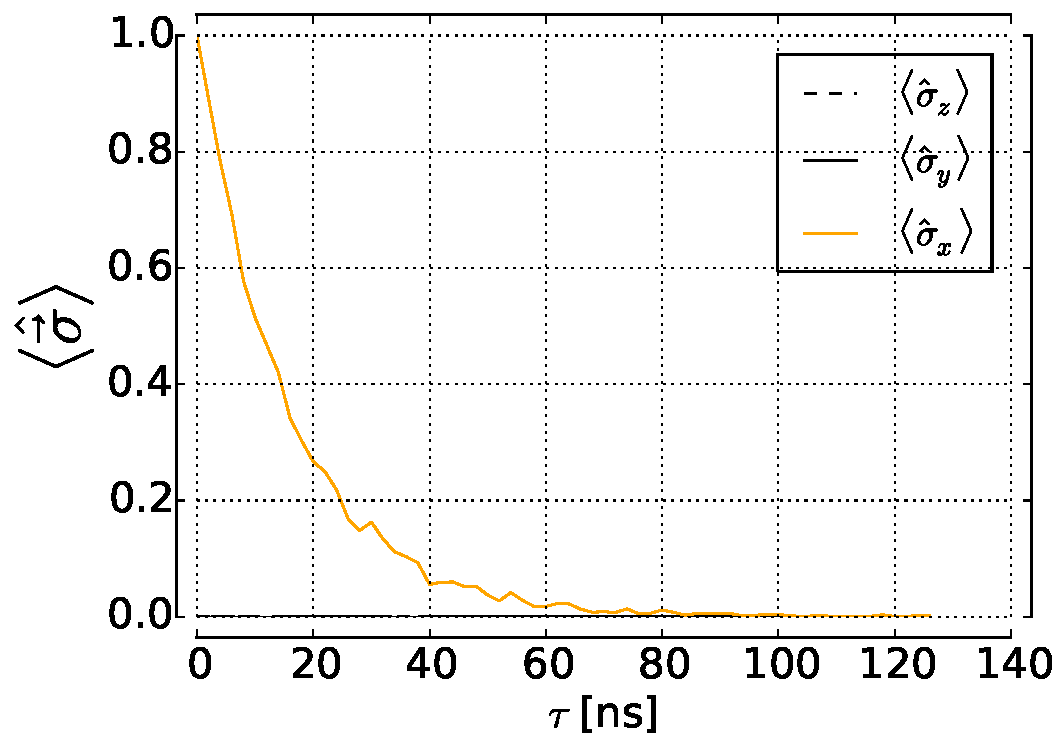
\includegraphics[width=\textwidth]{deph_white_se}
	
	Echo
	\end{columns}
	
	\vspace{0.2cm}
	\begin{itemize}
		\centering	
	\item \textbf{totally inefficient}, same for the master equation description
	\end{itemize}
	
}
\end{frame}

\section{Xmon cQED (QuTiP simulations)}


\subsection{Circuit quantization}
\frame{\frametitle{\secname}\framesubtitle{\subsecname}
Equivalent circuit for the transmon-resonator system:

\centering
\vspace{0.5cm}
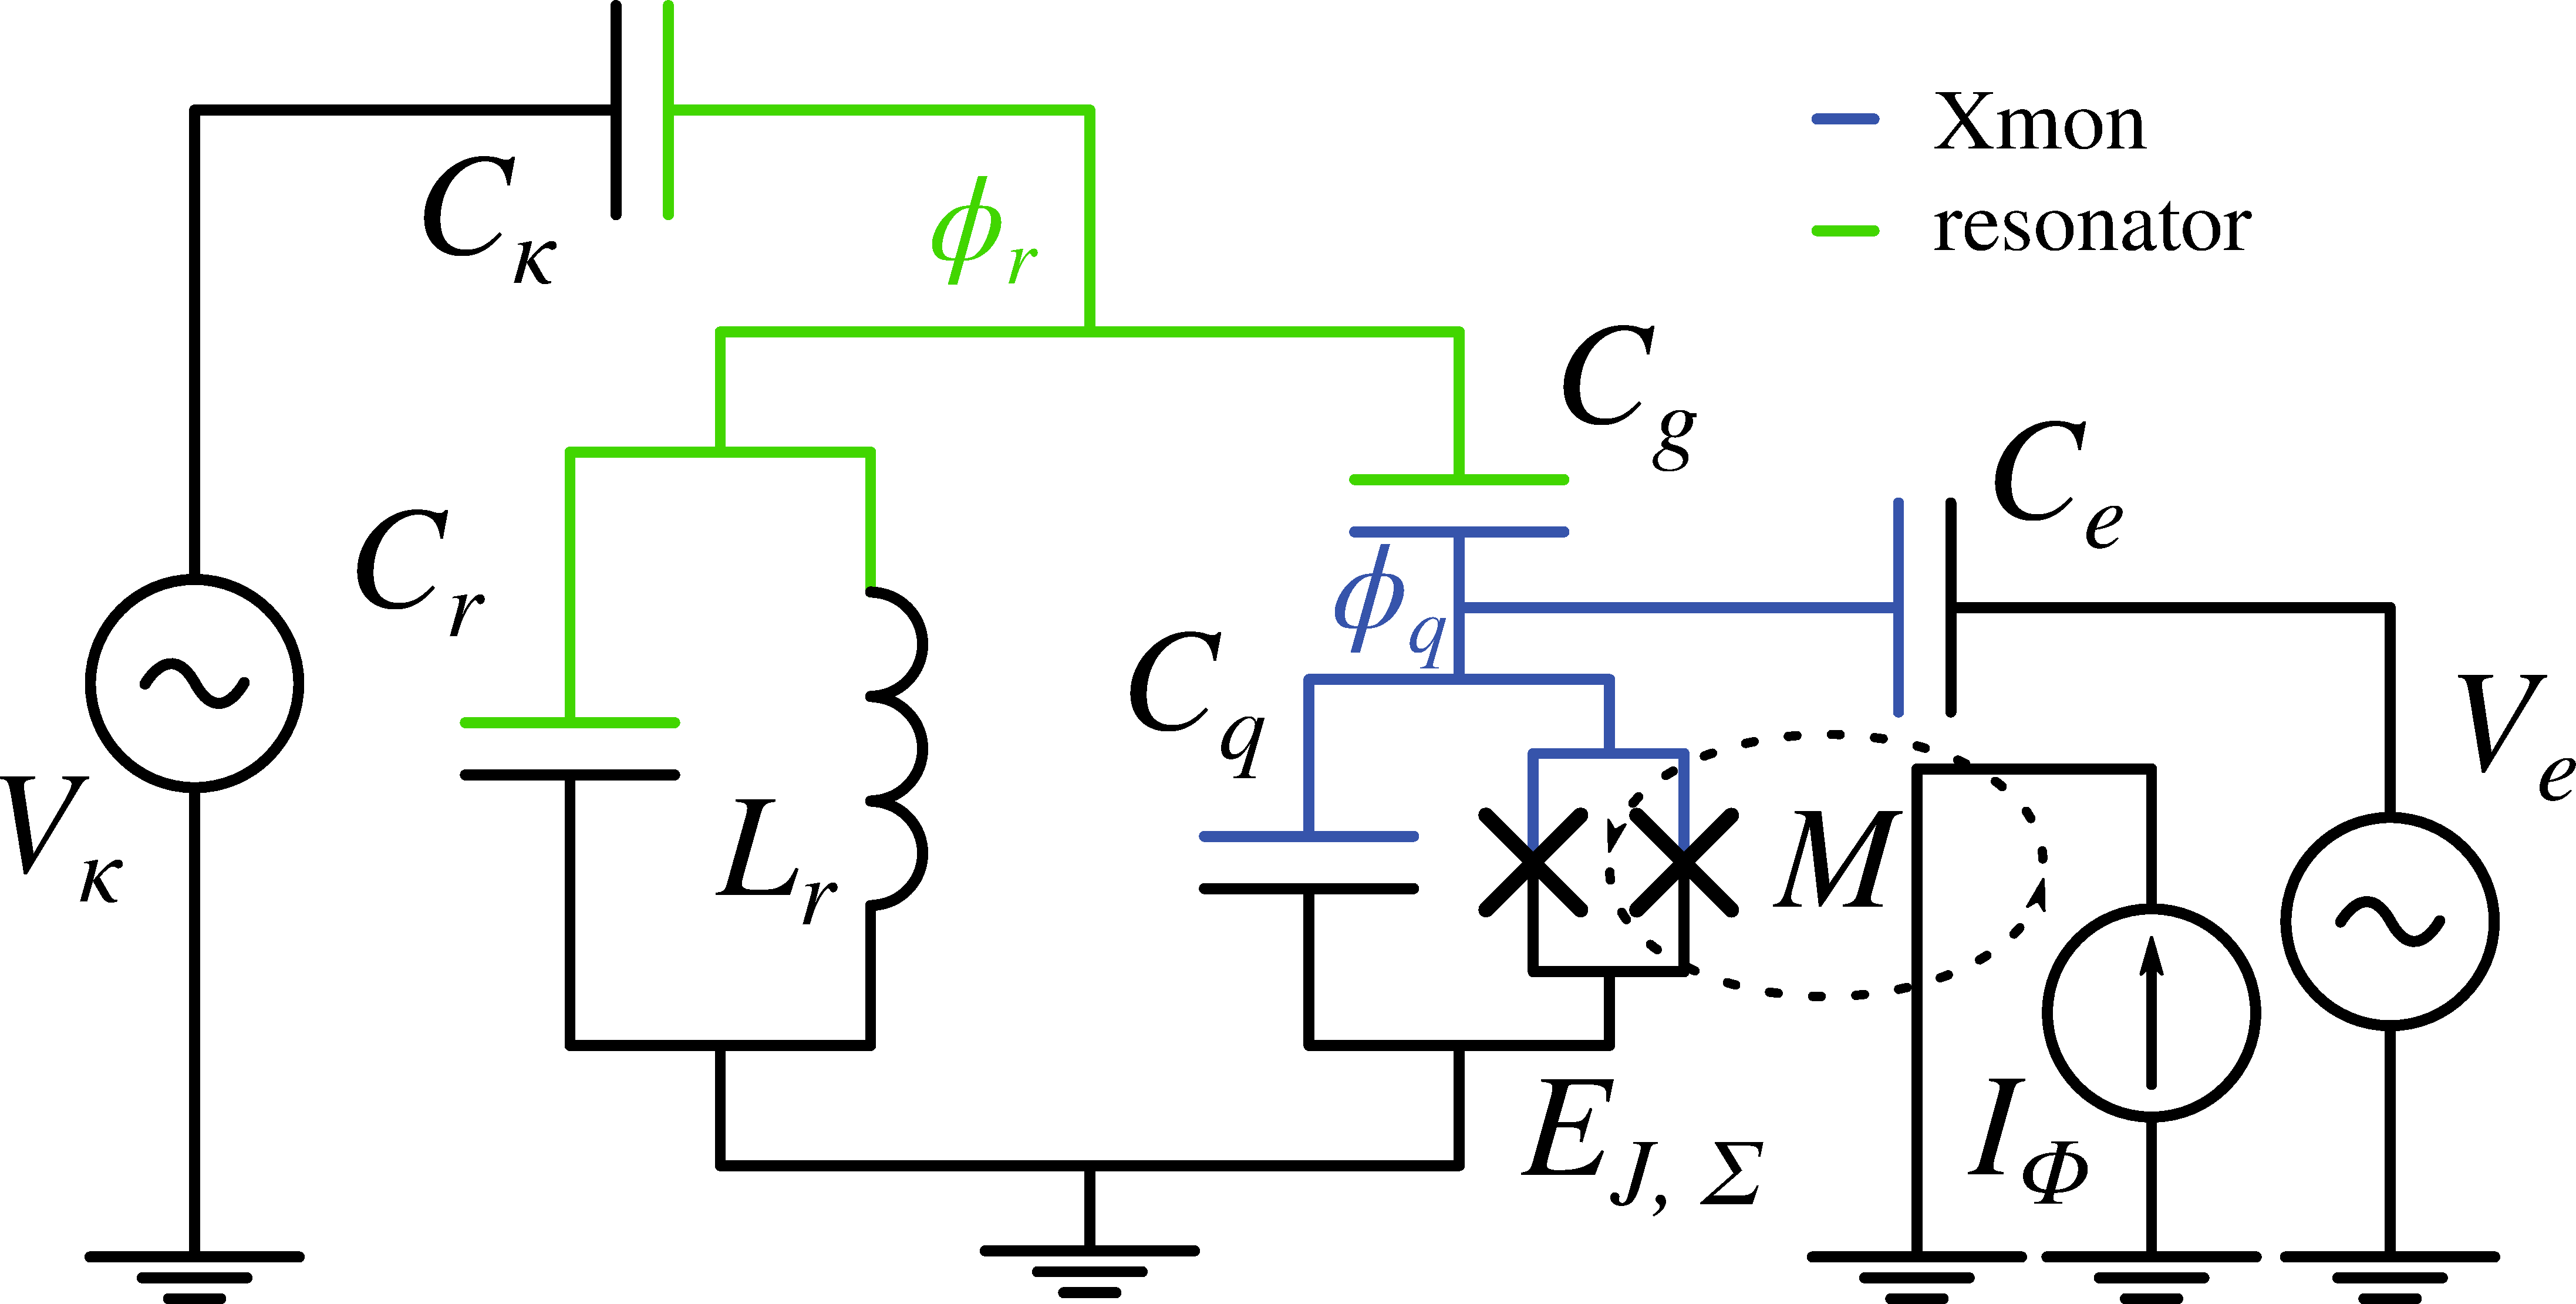
\includegraphics[width=0.8\textwidth]{xmon-resonator}
}

\frame{\frametitle{\secname}\framesubtitle{\subsecname}
\[
\begin{gathered}
\mathcal{\hat H} =  \underbrace{\frac{\hat \phi_r^2}{2 L_r} + \frac{(C_q+C_g) \hat Q_r^2}{2C_*^2}}_\text{resonator} 
+ \underbrace{\frac{(C_g + C_\kappa + C_r) \hat Q^2_q}{2C_*^2} - E_J (\Phi_{ext}) \cos \frac{2e}{\hbar}\hat \phi_q }_\text{qubit}
+ \underbrace{\frac{C_g\hat Q_r \hat Q_q}{C_*^2}}_\text{coupling} = \\
=  \hbar\omega_r\ \hat a^\dag \hat a \otimes \mathbbm{\hat 1}_q \quad (\mathcal{\hat H}_r) \\
+ 4 E_C\ \mathbbm{\hat 1}_r \otimes \hat n^2 - \frac{E_J(\Phi_{ext})}{2}\ \mathbbm{\hat 1}_r\otimes \sum_{n=-\infty}^{+\infty} \ket{n+1}\bra{n} + \ket{n}\bra{n+1} \quad (\mathcal{\hat H}_q) \\
- 2e \frac{C_g}{C_*} \sqrt{\frac{\hbar \omega_r }{2(C_q+C_g)}}\ i(\hat a^\dag - \hat a) \otimes \hat n, \quad (\mathcal{\hat H}_i)
\end{gathered}
\]
}

\subsection{Cooper pair distribution for an isolated Xmon}
\frame{\frametitle{\secname}\framesubtitle{\subsecname}
\begin{columns}[c]
\column{0.5\textwidth}
\centering
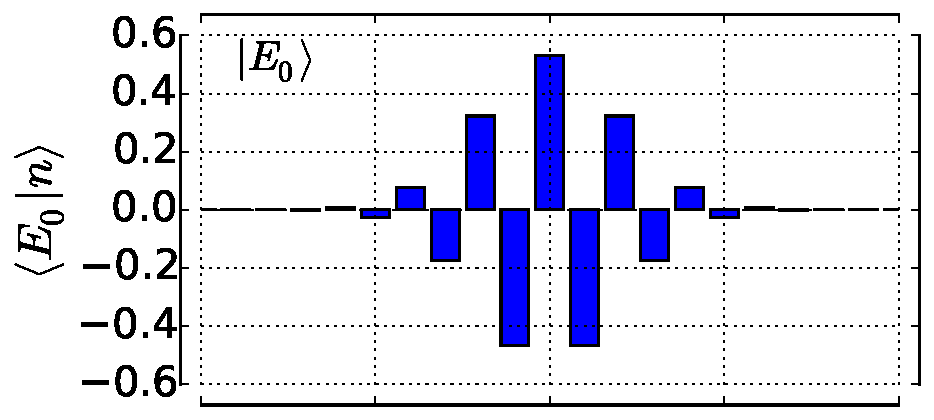
\includegraphics[width=\textwidth]{tr_CPD_0}

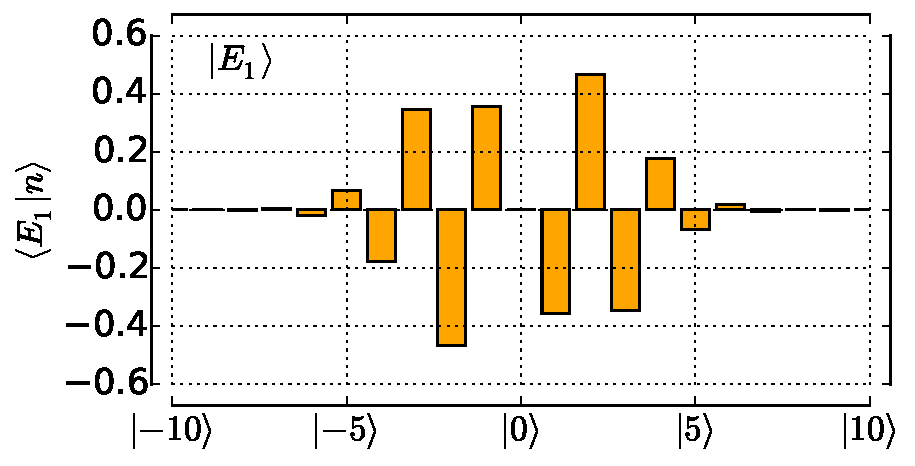
\includegraphics[width=\textwidth]{tr_CPD_1}
\column{0.5\textwidth}
\centering
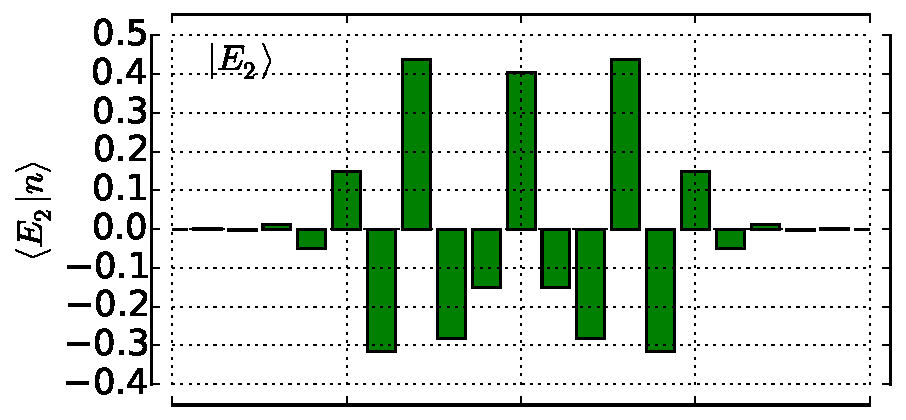
\includegraphics[width=\textwidth]{tr_CPD_2}

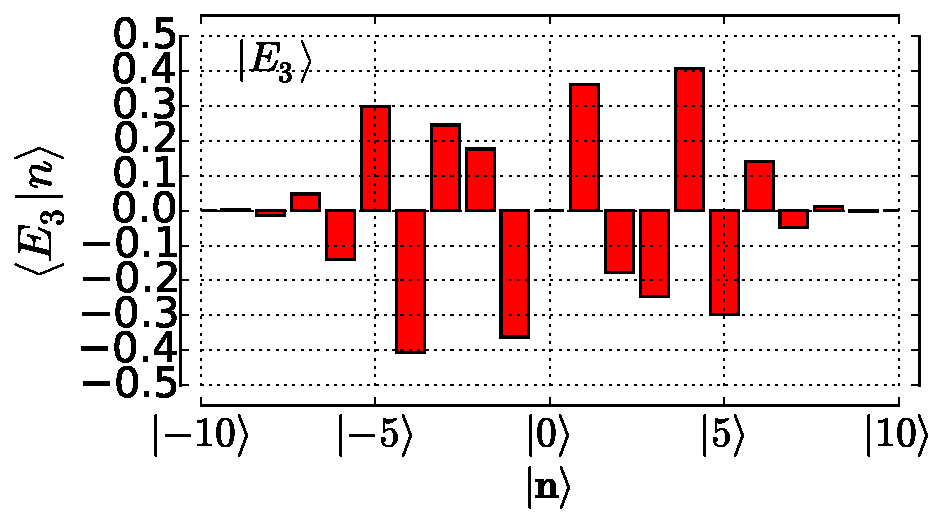
\includegraphics[width=\textwidth]{tr_CPD_3}
\end{columns}

}


\frame[c]{\frametitle{\secname}\framesubtitle{\subsecname}
For weak driving the two-level dynamics is preserved ($\ket{\psi(t)}= \sum_k c_k(t) \ket{E_k}$):

\begin{columns}[c]
\column{0.5\textwidth}
\centering
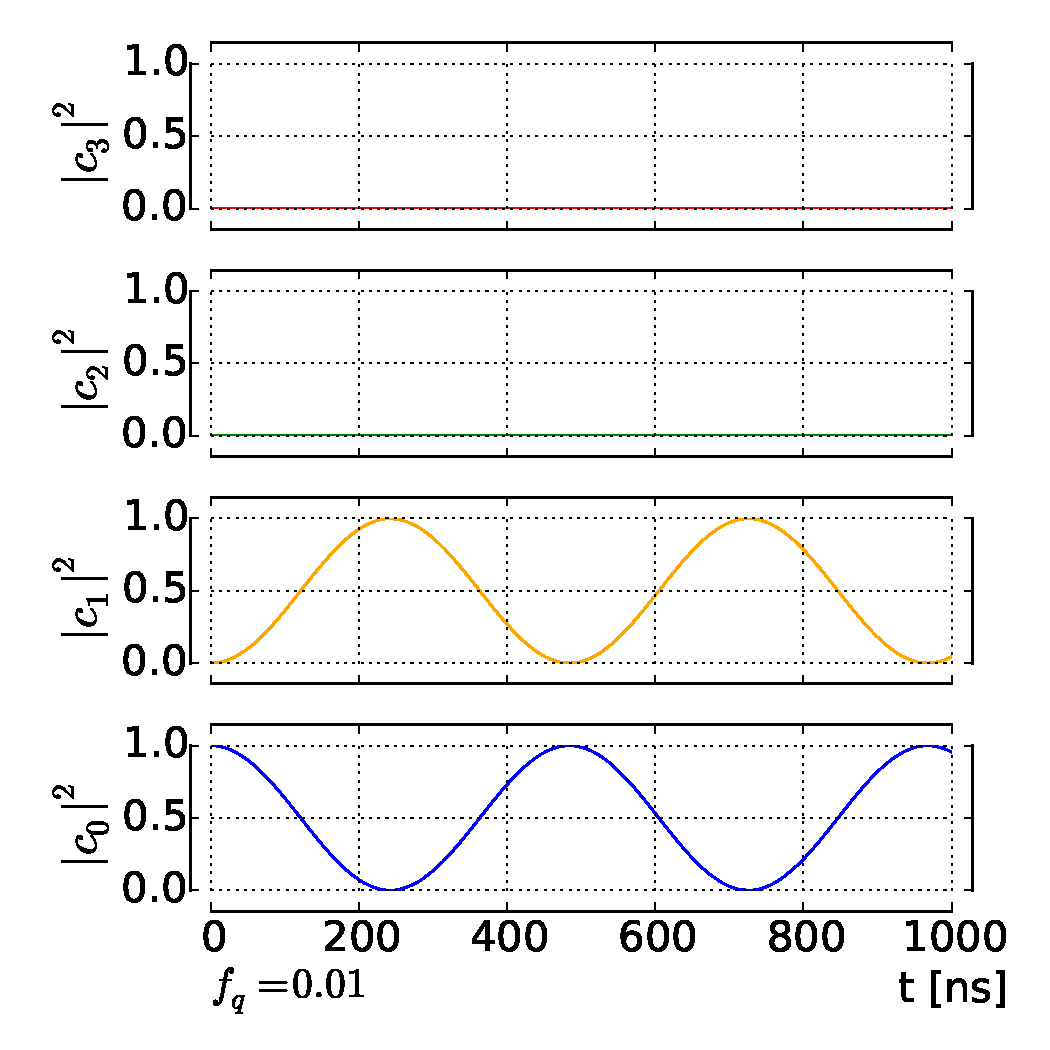
\includegraphics[width=\textwidth]{tr_weak_dr}
\column{0.5\textwidth}
\centering
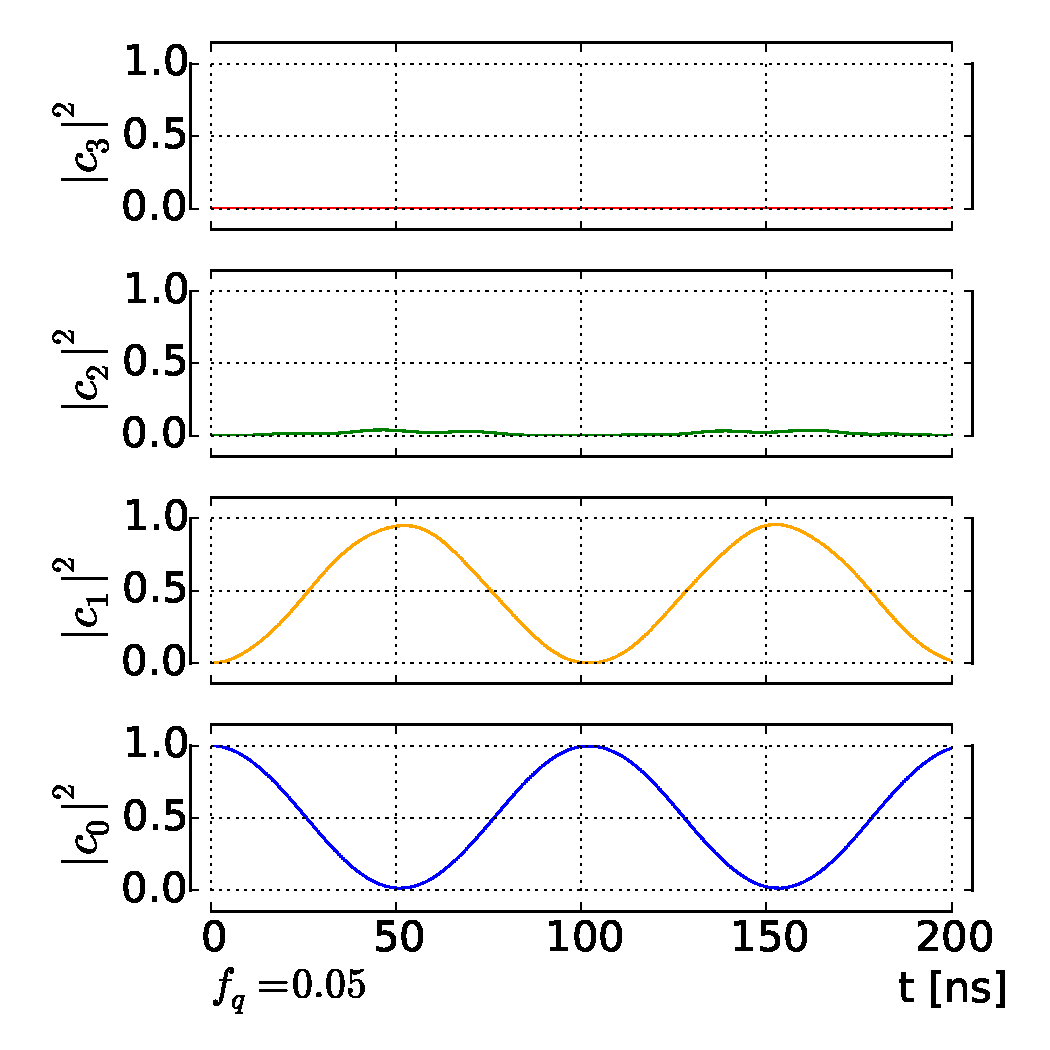
\includegraphics[width=\textwidth]{tr_int_dr}
\end{columns}
}

\frame[c]{\frametitle{\secname}\framesubtitle{\subsecname}
But not for the strong drive ($\ket{\psi(t)} = \sum_k c_k(t) \ket{E_k}$):

\begin{columns}[c]
\column{0.5\textwidth}
\centering
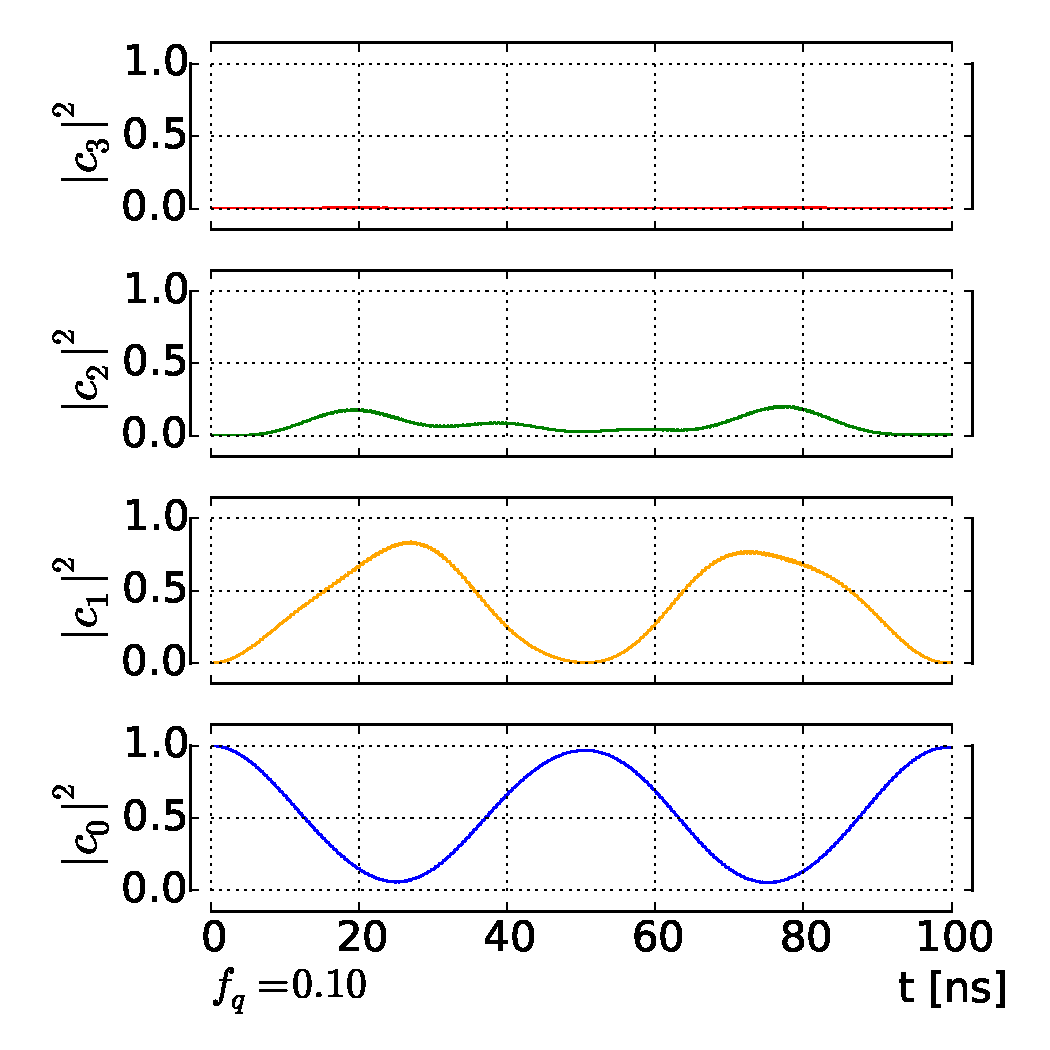
\includegraphics[width=\textwidth]{tr_str_dr}
\column{0.5\textwidth}
\centering
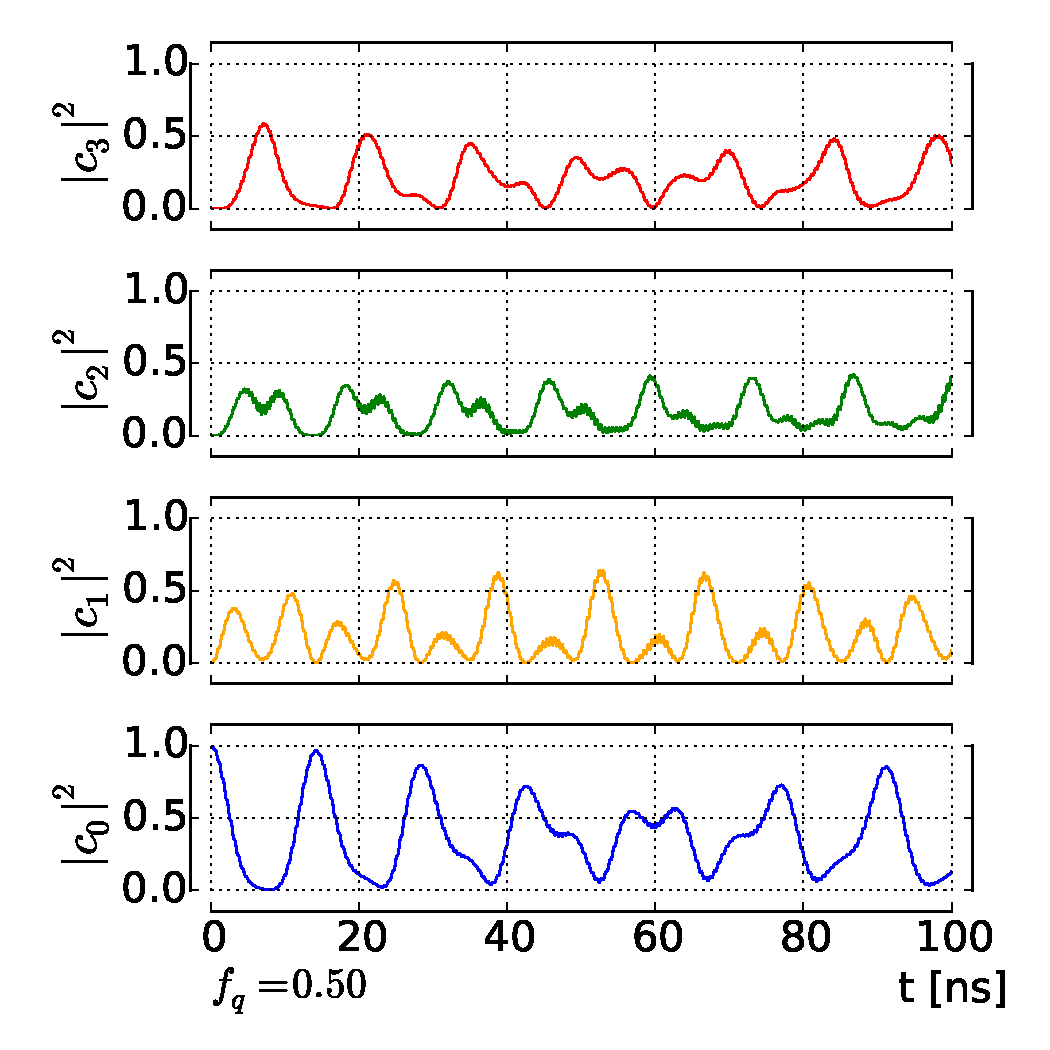
\includegraphics[width=\textwidth]{tr_vstr_dr}
\end{columns}
}


\subsection{Eigenproblem for a qubit-resonator system}
\frame{\frametitle{\secname}\framesubtitle{\subsecname}
Energy level structure:

\vspace{0.5cm}
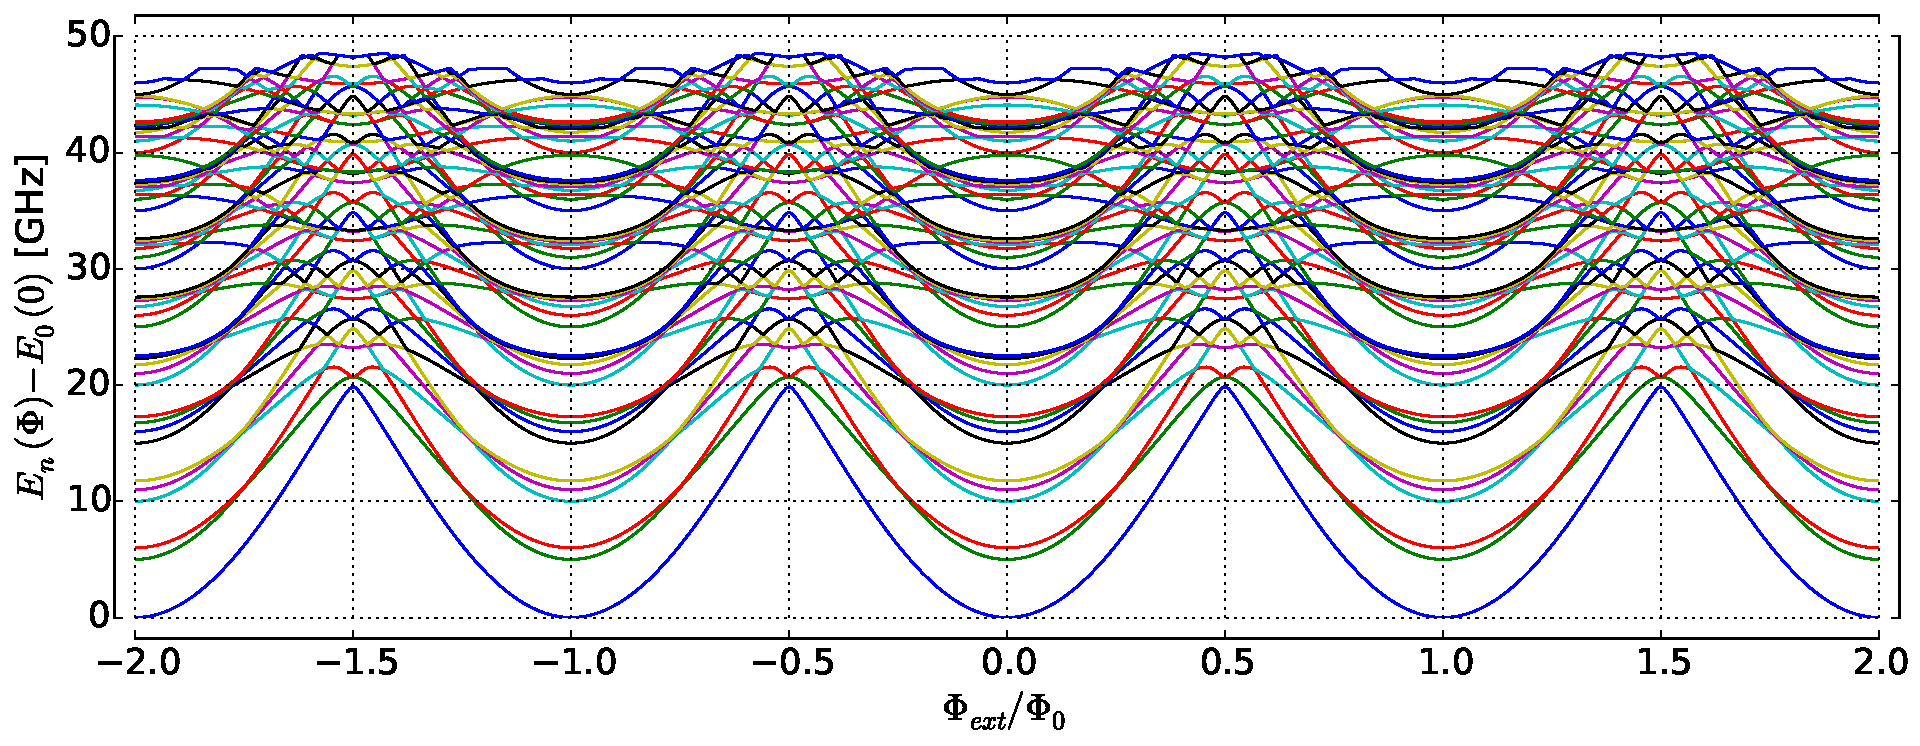
\includegraphics[width=\textwidth]{levels.pdf}
}

\frame{\frametitle{\secname}\framesubtitle{\subsecname}
Frequencies $f_{0n} = (E_n - E_0)/h$ for $\omega_q > \omega_r$:

\vspace{0.5cm}
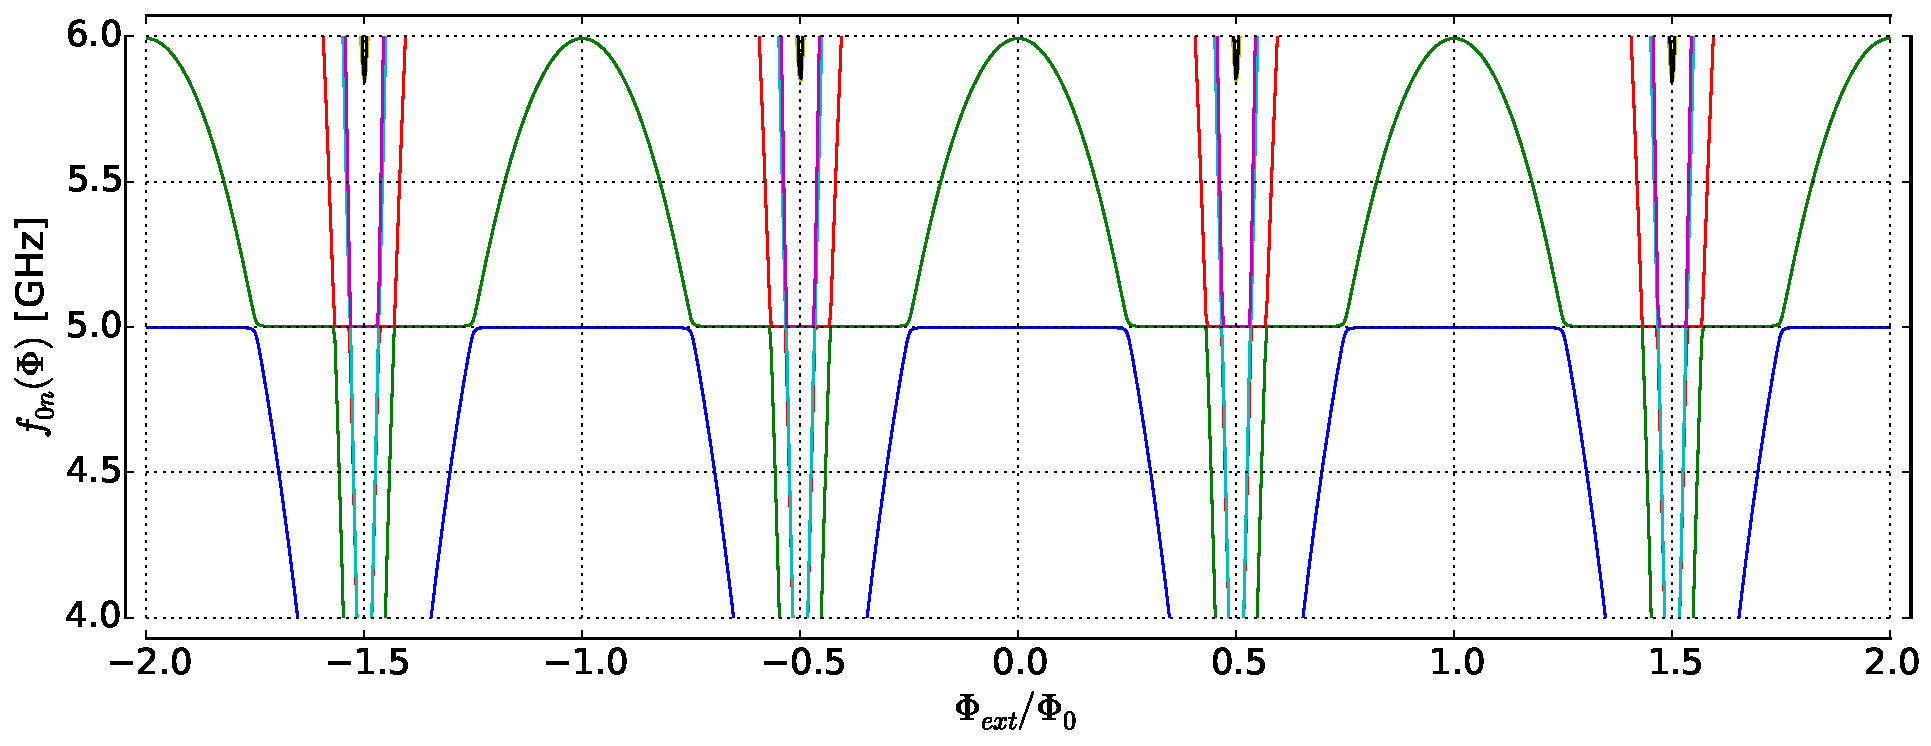
\includegraphics[width=\textwidth]{freqs.pdf}
}

\subsection{Dispersive shifts}
\frame{\frametitle{\secname}\framesubtitle{\subsecname} 
Dispersive shifts originate from the level structure of the whole composite system:

\vspace{0.1cm}
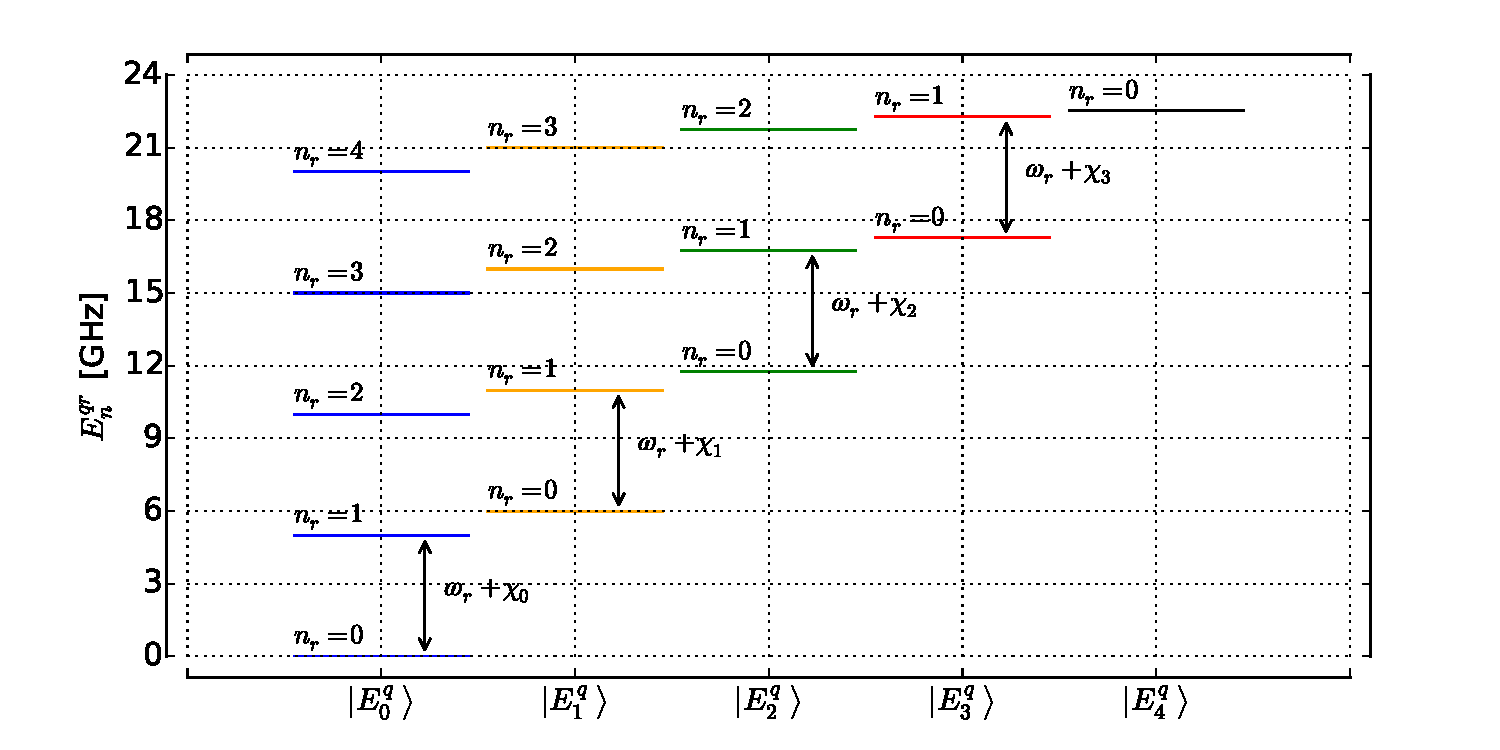
\includegraphics[height=0.8\textheight]{diagram}
}

\frame{\frametitle{\secname}\framesubtitle{\subsecname} 
It's possible to determine these shifts with high accuracy using the second order perturbation theory:
\begin{gather*}
\chi_0 = g^2\sbrkt{\frac{n_{ge}^2}{\omega_r - \omega_{ge}}-\frac{n_{ge}^2}{\omega_r + \omega_{ge}}},\\
\chi_1 = g^2\sbrkt{\frac{n_{ef}^2}{\omega_r - \omega_{ef}} - \frac{n_{ef}^2}{\omega_r + \omega_{ef}} + \frac{n_{eg}^2}{\omega_r + \omega_{ge}}-\frac{n_{eg}^2}{\omega_r - \omega_{ge} }},\\
\chi_2 = g^2\sbrkt{\frac{n_{fd}^2}{\omega_r - \omega_{fd}} -\frac{n_{fd}^2}{\omega_r + \omega_{fd}} + \frac{n_{fe}^2}{\omega_r + \omega_{ef}}- \frac{n_{fe}^2}{\omega_r -\omega_{ef}}}.
\end{gather*}
}

\frame{\frametitle{\secname}\framesubtitle{\subsecname} 
The shifts depend on the detuning  $\Delta_\omega = \omega_r - \omega_{ge}$ and  $\Phi_{ext}$:

\vspace{0.5cm}
\begin{columns}[c]
\column{0.5\textwidth}
\centering
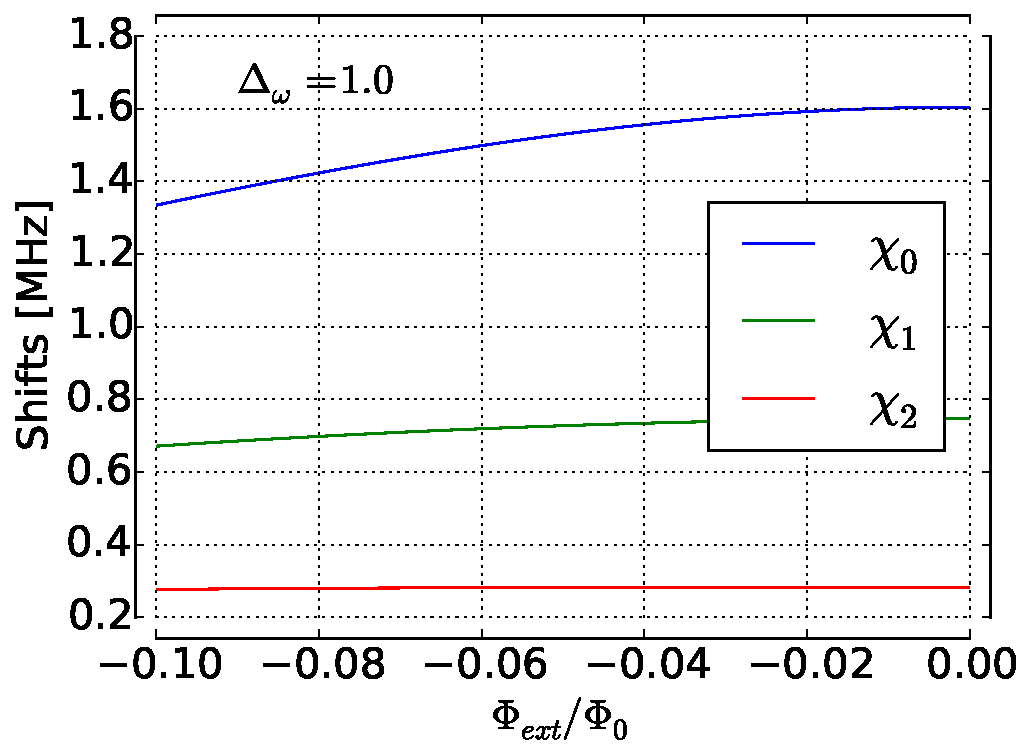
\includegraphics[height=0.65\textheight]{shifts10}
\column{0.5\textwidth}
\centering
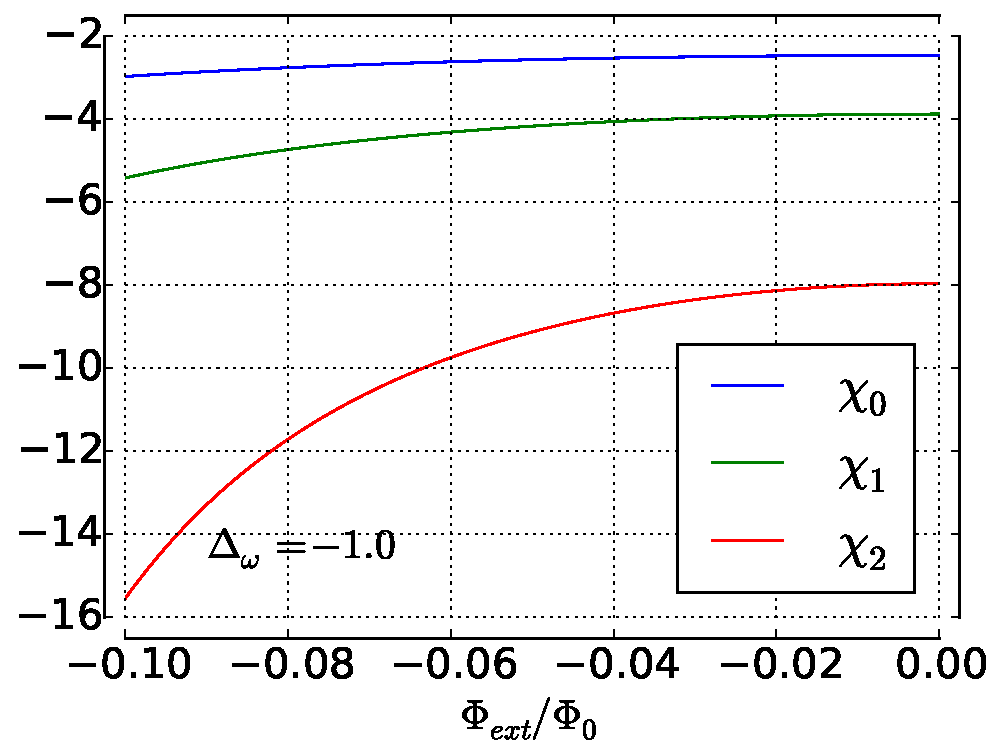
\includegraphics[height=0.65\textheight]{shifts-10}

\end{columns}
}

\section*{Final words}
\subsection*{Summary}
\frame{\frametitle{\secname}\framesubtitle{\subsecname} 
\begin{columns}[c]
\column{0.5\textwidth}
\begin{itemize}
\item \textbf{Quality factors} and \textbf{coupling capacitance} calculations, simulations of \textbf{CPW resonators} and \textbf{extraction of capacitances} using Sonnet
\item Investigation of \textbf{classical} and \textbf{quantum noise} influence on the qubit, numerical simulations of the \textbf{pure dephasing under different types of noise}
\item \textbf{Quantization of Xmon-resonator} circuit to transform capacitances and quality factors to the \textbf{coupling strengths, driving amplitudes} and \textbf{decay rates} 
\end{itemize}
\column{0.5\textwidth}
\centering

\hspace{-0.2cm} 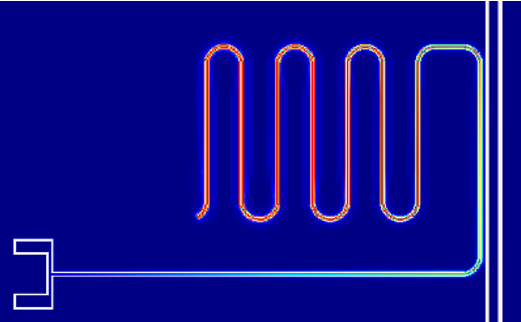
\includegraphics[height=0.2\textheight]{xmonres_sim_claw_h}

\vspace{0.1cm}
\hspace{-0.7cm}	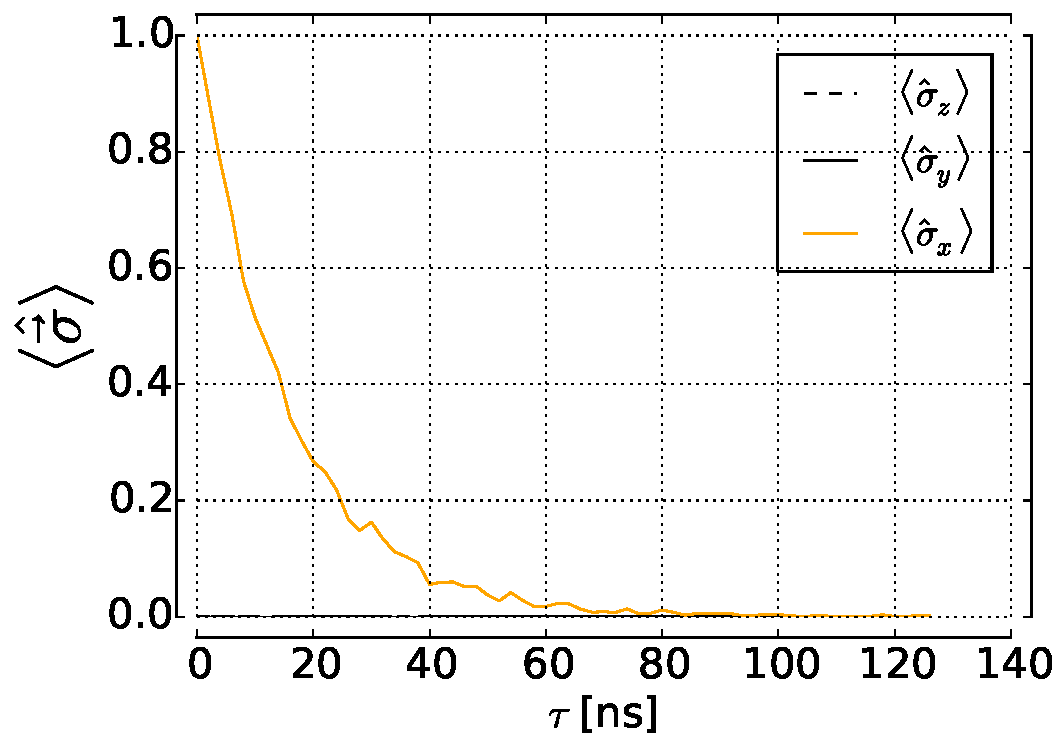
\includegraphics[height=0.3\textheight]{deph_white_se}

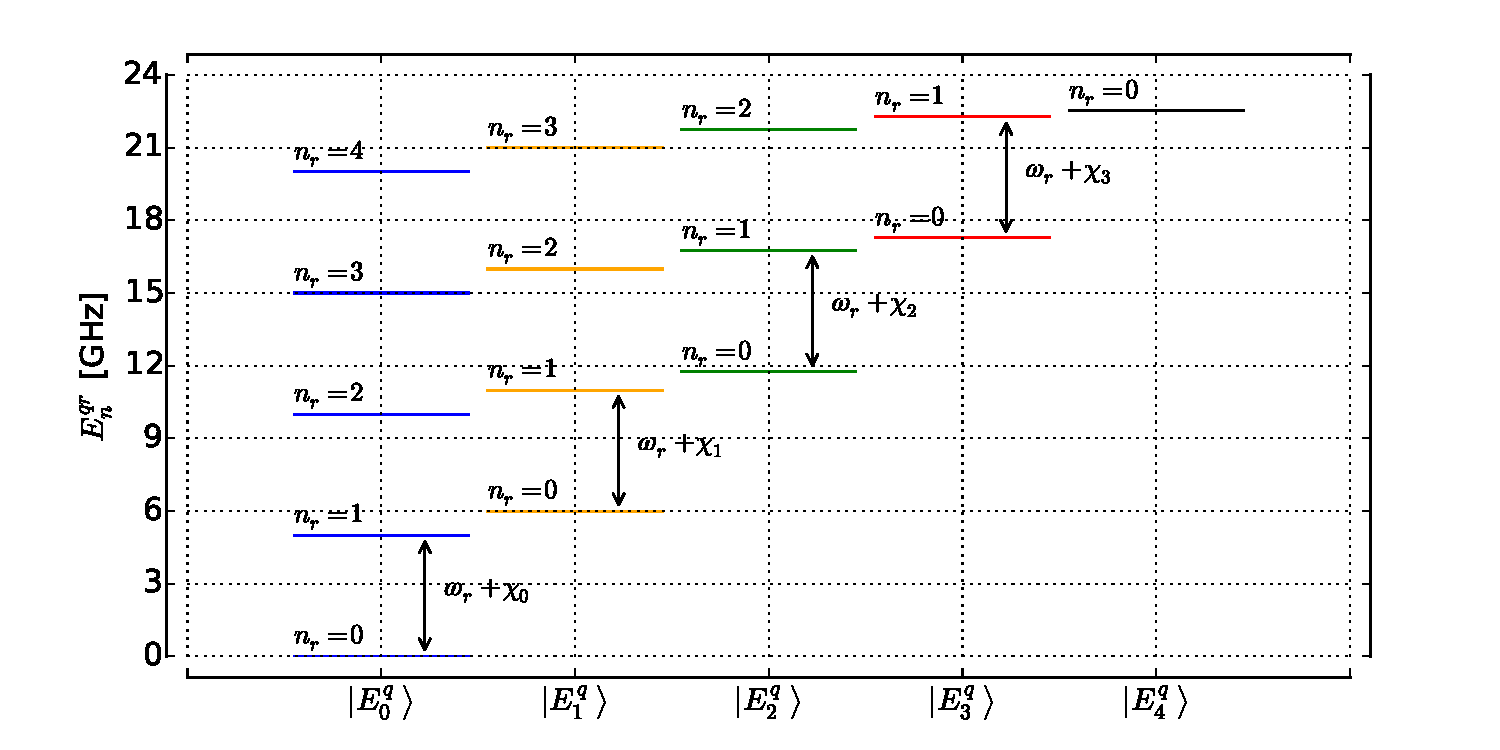
\includegraphics[height=0.3\textheight]{diagram}
\end{columns}
}

\appendix

\subsection*{Acknowledgements}
\frame[c]{\frametitle{\secname}\framesubtitle{\subsecname} 

{\large
\begin{itemize}
\centering
\item A. V. Ustinov

\vspace{0.5cm}
\item J. Lisenfeld and A. Bilmes
\end{itemize}
}
}
\frame[c]{\frametitle{\secname}\framesubtitle{\subsecname} 
\begin{center}
{\huge Thank you!}
\end{center}
}

\end{document}